%! TeX program = lualatex
\documentclass[a4paper,11pt]{article} 
% packages
\usepackage{censor}
\StopCensoring
\usepackage{fontspec}
\usepackage{tcolorbox}
\setmainfont{EB Garamond}
% for tironian et fallback
% % \directlua{luaotfload.add_fallback
% % ("emojifallback",
% %      {"Noto Serif:mode=harf"}
% % )}
% % \setmainfont{EB Garamond}[RawFeature={fallback=emojifallback}]

\setmonofont[Scale=MatchLowercase]{Deja Vu Sans Mono}
\usepackage[a4paper,left=2cm,right=2cm,top=\dimexpr15mm+1.5\baselineskip,bottom=2cm]{geometry}
\setlength{\parindent}{0pt}

\usepackage{ulem}
\usepackage{gensymb}
\usepackage{fancyhdr}       % Headers and footers 
\fancyhead[R]{\normalfont \leftmark}
\fancyhead[L]{}
\pagestyle{fancy}

\usepackage{microtype}      % Slightly tweak font spacing for aesthetics
\usepackage[english]{babel} % Language hyphenation and typographical rules
\usepackage{xcolor}
\definecolor{linkblue}{RGB}{0, 64, 128}
\usepackage[final, colorlinks = false, urlcolor = linkblue]{hyperref} 
% \newcommand{\secref}[1]{\textbf{§~\nameref{#1}}}
\newcommand{\secref}[1]{\textbf{§\ref{#1}~\nameref{#1}}}
\usepackage{multicol}
\usepackage{amsmath}
\usepackage{amssymb}

\usepackage{changepage}     % adjust margins on the fly

\usepackage{minted}
\usemintedstyle{algol_nu}

\usepackage{pgfplots}
\pgfplotsset{width=\textwidth,compat=1.9}

\usepackage{caption}
\newenvironment{code}{\captionsetup{type=listing}}{}
\captionsetup[listing]{skip=0pt}
\setlength{\abovecaptionskip}{5pt}
\setlength{\belowcaptionskip}{5pt}

\usepackage[yyyymmdd]{datetime}
\renewcommand{\dateseparator}{--}

\usepackage{enumitem}

\usepackage{titlesec}

\author{Andrew Hayes}

\begin{document}
\begin{titlepage}
    \begin{center}
        \hrule
        \vspace*{0.6cm}
        \censor{\huge \textbf{CT404}}
        \vspace*{0.6cm}
        \hrule
        \LARGE
        \vspace{0.5cm}
            Graphics \& Image Processing
        \vspace{0.5cm}
        \hrule

        \vfill
            \centering
            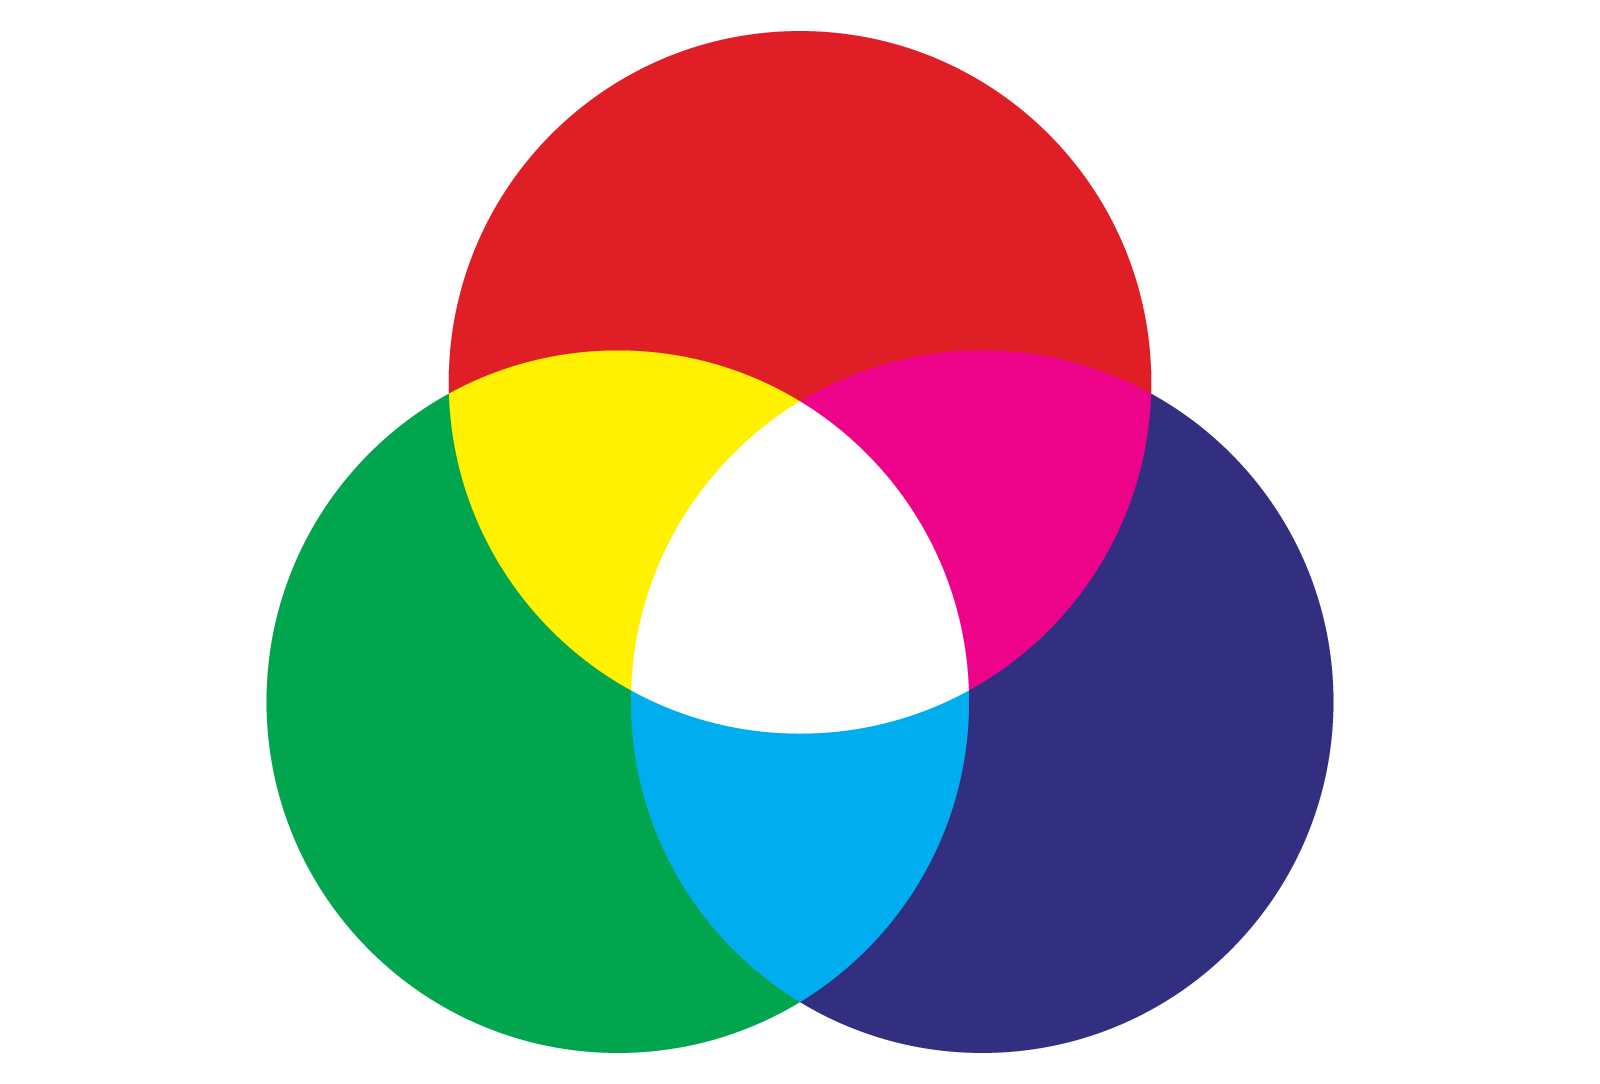
\includegraphics[width=\textwidth]{images/cover.png}
        \vfill

        \hrule
        \begin{minipage}{0.495\textwidth} 
            \vspace{0.4em}
            \raggedright
            \normalsize 
            Name: \censor{Andrew Hayes} \\
            E-mail: \censor{\href{mailto://a.hayes18@universityofgalway.ie}{\texttt{a.hayes18@universityofgalway.ie}}}  \hfill\\   
            Student ID: \censor{21321503} \hfill
        \end{minipage}
        \begin{minipage}{0.495\textwidth} 
            \raggedleft
            \vspace*{0.8cm}
            \Large
            \today
            \vspace*{0.6cm}
        \end{minipage}
        \medskip\hrule 
    \end{center}
\end{titlepage}

\pagenumbering{roman}
\newpage
\tableofcontents
\newpage
\setcounter{page}{1}
\pagenumbering{arabic}

\section{Introduction}
Textbooks:
\begin{itemize}
    \item   Main textbook: \textit{Image Processing and Analysis} -- Stan Birchfield (ISBN: 978-1285179520).
    \item   \textit{Introduction to Computer Graphics} -- David J. Eck. (Available online at \url{https://math.hws.edu/graphicsbook/}).
    \item   \textit{Computer Graphics: Principles and Practice} -- John F. Hughes et al. (ISBN: 0-321-39952-8).
    \item   \textit{Computer Vision: Algorithms and Applications} -- Richard Szeliski (ISBN: 978-3-030-34371-2).
\end{itemize}

\textbf{Computer graphics} is the processing \& displaying of images of objects that exist conceptually rather than
physically with emphasis on the generation of an image from a model of the objects, illumination, etc. and the
real-time rendering of images.
Ideas from 2D graphics extend to 3D graphics.
\\\\
\textbf{Digital Image processing/analysis} is the processing \& display of images of real objects, with an emphasis
on the modification and/or analysis of the image in order to automatically or semi-automatically extract useful
information.
Image processing leads to more advanced feature extraction \& pattern recognition techniques for image analysis \&
understanding.

\subsection{Grading}
\begin{itemize}
    \item   Assignments: 30\%.
    \item   Final Exam: 70\%.
\end{itemize}

\subsubsection{Reflection on Exams}
``A lot of people give far too little detail in these questions, and/or don't address the discussion 
parts -- they just give some high-level definitions and consider it done -- which isn't enough for 
final year undergrad, and isn't answering the question.
More is expected in answers than just repeating what's in my slides. 
The top performers demonstrate a higher level of understanding and synthesis as well as more 
detail about techniques and discussion of what they do on a technical level and how they fit 
together''

\subsection{Lecturer Contact Information}
\begin{multicols}{2}
    \begin{itemize}
        \item   Dr. Nazre Batool.
        \item   \href{mailto://nazre.batool@universityofgalway.ie}{\texttt{nazre.batool@universityofgalway.ie}}
        \item   Office Hours: Thursdays 16:00 -- 17:00, CSB-2009.

        \item   Dr. Waqar Shahid Qureshi.
        \item   \href{mailto://waqarshahid.qureshi@universityofgalway.ie}{\texttt{waqarshahid.qureshi@universityofgalway.ie}}.
        \item   Office Hours: Thursdays 16:00 -- 17:00, CSB-3001.
    \end{itemize}
\end{multicols}

\section{Introduction to 2D Graphics}
\subsection{Digital Images -- Bitmaps}
\textbf{Bitmaps} are grid-based arrays of colour or brightness (greyscale) information.
\textbf{Pixels} (\textit{picture elements}) are the cells of a bitmap.
The \textbf{depth} of a bitmap is the number of bits-per-pixel (bpp).

\subsection{Colour Encoding Schemes}
Colour is most commonly represented using the \textbf{RGB (Red, Green, Blue)} scheme, typically using 24-bit colour
with one 8-bit number representing the level of each colour channel in that pixel.
\\\\
Alternatively, images can also be represented in \textbf{greyscale} wherein pixels are represented with one
(typically 8-bit) brightness value (or scale of grey) .

\subsection{The Real-Time Graphics Pipeline}
\begin{figure}[H]
    \centering
    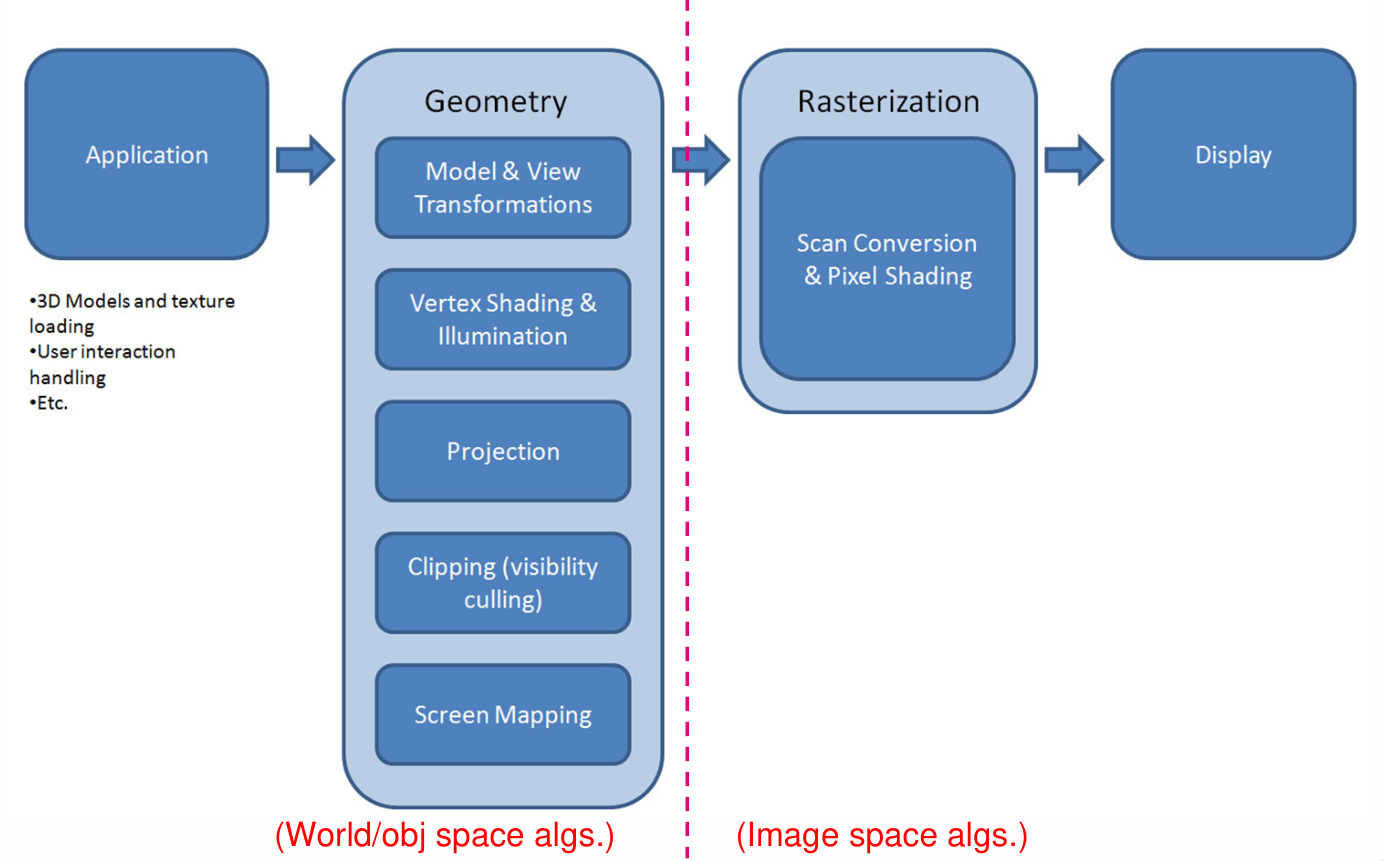
\includegraphics[width=\textwidth]{images/real_time_graphics_pipeline.png}
    \caption{The Real-Time Graphics Pipeline}
\end{figure}

\subsection{Graphics Software}
The \textbf{Graphics Processing Unit (GPU)} of a computer is a hardware unit designed for digital image processing \& to 
accelerate computer graphics that is included in modern computers to complement the CPU.
They have internal, rapid-access GPU memory and parallel processors for vertices \& fragments to speed up graphics 
renderings.
\\\\
\textbf{OpenGL} is a 2D \& 3D graphics API that has existed since 1992 that is supported by the graphics hardware in most
computing devices today.
\textbf{WebGL} is a web-based implementation of OpenGL for use within web browsers.
OpenGL ES for Embedded Systems such as tablets \& mobile phones also exists.
\\\\
OpenGL was originally a client/server system with the CPU+Application acting as a client sending commands \& data to the GPU
acting as a server.
This was later replaced by a programmable graphics interface (OpenGL 3.0) to write GPU programs (shaders) to be run by the 
GPU directly.
It is being replaced by newer APIs such as Vulkan, Metal, \& Direct3D and WebGL is being replaced by WebGPU.

\subsection{Graphics Formats}
\textbf{Vector graphics} are images described in terms of co-ordinate drawing operations, e.g. AutoCAD, PowerPoint, Flash, 
SVG.
\textbf{SVG (Scalable Vector Graphics)} is an image specified by vectors which are scalable without losing any quality.
\\\\
\textbf{Raster graphics} are images described as pixel-based bitmaps.
File formats such as GIF, PNG, JPEG represent the image by storing colour values for each pixel.

\section{2D Vector Graphics}
\textbf{2D vector graphics} describe drawings as a series of instructions related to a 2-dimensional co-ordinate system.
Any point in this co-ordinate system can be specified using two numbers $(x, y)$:
\begin{itemize}
    \item   The horizontal component $x$, measuring the distance from the left-hand edge of the screen or window.
    \item   The vertical component $y$, measuring the distance from the bottom of the screen or window (or sometimes from the
            top).
\end{itemize}

\subsection{Transformations}
\subsubsection{2D Translation}
The \textbf{translation} of a point in 2 dimensions is the movement of a point $(x,y)$ to some other point $(x', y')$.
$$
x' = x + a
$$
$$
y' = y + b
$$

\begin{figure}[H]
    \centering
    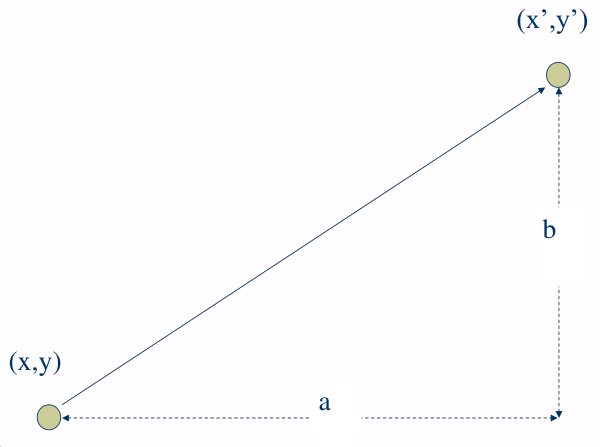
\includegraphics[width=0.5\textwidth]{images/2d_translation.png}
    \caption{2D Translation of a Point}
\end{figure}

\subsubsection{2D Rotation of a \textit{Point}}
The simplest rotation of a point around the origin is given by:
$$
x' = x \cos \theta - y \sin \theta
$$
$$
y' = x \cos \theta + y \sin \theta
$$

\begin{figure}[H]
    \centering
    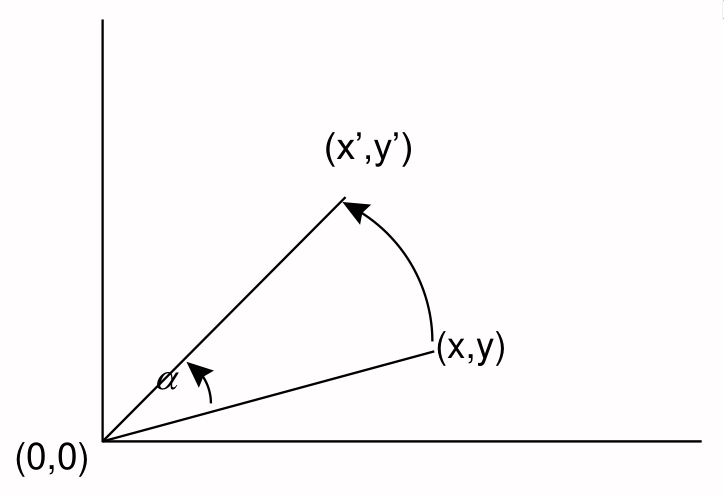
\includegraphics[width=0.5\textwidth]{images/2d_point_rotation.png}
    \caption{2D Rotation of a Point}
\end{figure}

\subsubsection{2D Rotation of an \textit{Object}}
In vector graphics, \textbf{objects} are defined as series of drawing operations (e.g., straight lines) performed on a set 
of vertices.
To rotate a line or more complex object, we simply apply the equations to rotate a point to the $(x,y)$ co-ordinates of each 
vertex.

\begin{figure}[H]
    \centering
    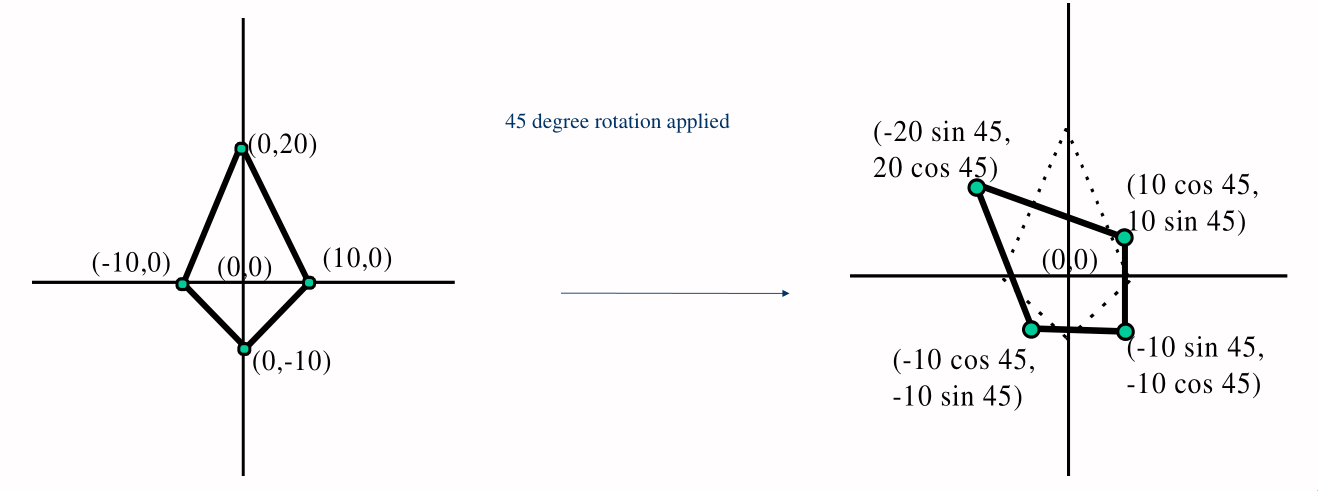
\includegraphics[width=0.7\textwidth]{images/2d_object_rotation.png}
    \caption{2D Rotation of an Object}
\end{figure}

\subsubsection{Arbitrary 2D Rotation}
In order to rotate around an arbitrary point $(a,b)$, we perform translation, then rotation, then reverse the translation.
$$
x' = a + (x - a) \cos \theta - (y - b) \sin \theta
$$
$$
y' = a + (x - a) \cos \theta + (y - b) \sin \theta
$$

\begin{figure}[H]
    \centering
    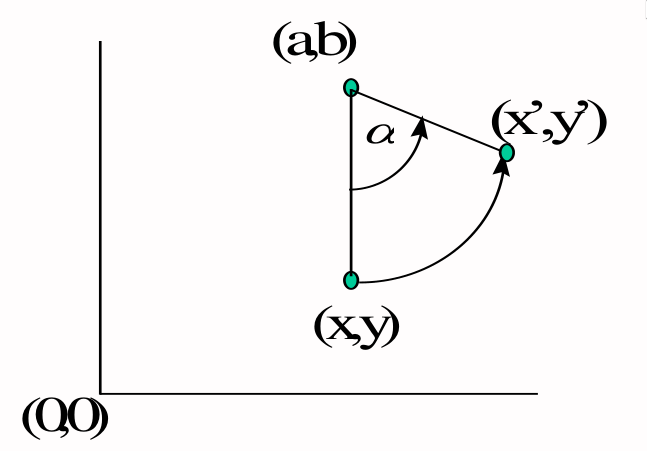
\includegraphics[width=0.5\textwidth]{images/2d_arbitrary_rotation.png}
    \caption{Arbitrary 2D Rotation}
\end{figure}

\subsubsection{Matrix Notation}
\textbf{Matrix notation} is commonly used for vector graphics as more complex operations are often easier in matrix format 
and because several operations can be combined easily into one matrix using matrix algebra.

Rotation about $(0,0)$:
$$
\begin{bmatrix}
    x' & y'
\end{bmatrix}
=
\begin{bmatrix}
    x & y
\end{bmatrix}
\begin{bmatrix}
 \cos \theta & \sin \theta \\
-\sin \theta & \cos \theta
\end{bmatrix}
$$

Translation:
$$
\begin{bmatrix}
    x' & y' 1
\end{bmatrix}
=
\begin{bmatrix}
    x & y & 1
\end{bmatrix}
\begin{bmatrix}
    1 & 0 & 0 \\
    0 & 1 & 0 \\
    a & 0 & 1
\end{bmatrix}
$$

\subsubsection{Scaling}
\textbf{Scaling} of an object is achieved by considering each of its vertices in turn, multiplying said vertex's $x$ \& $y$
values by the scaling factor.
A scaling factor of 2 will double the size of the object, while a scaling factor of 0.5 will halve it.
It is possible to have different scaling factors for $x$ \& $y$, resulting in a \textbf{stretch}:
$$
x' = x \times s
$$
$$
y' = y \times t
$$

If the object is not centred on the origin, then scaling it will also effect a translation.

\subsubsection{Order of Transformations}
\begin{figure}[H]
    \centering
    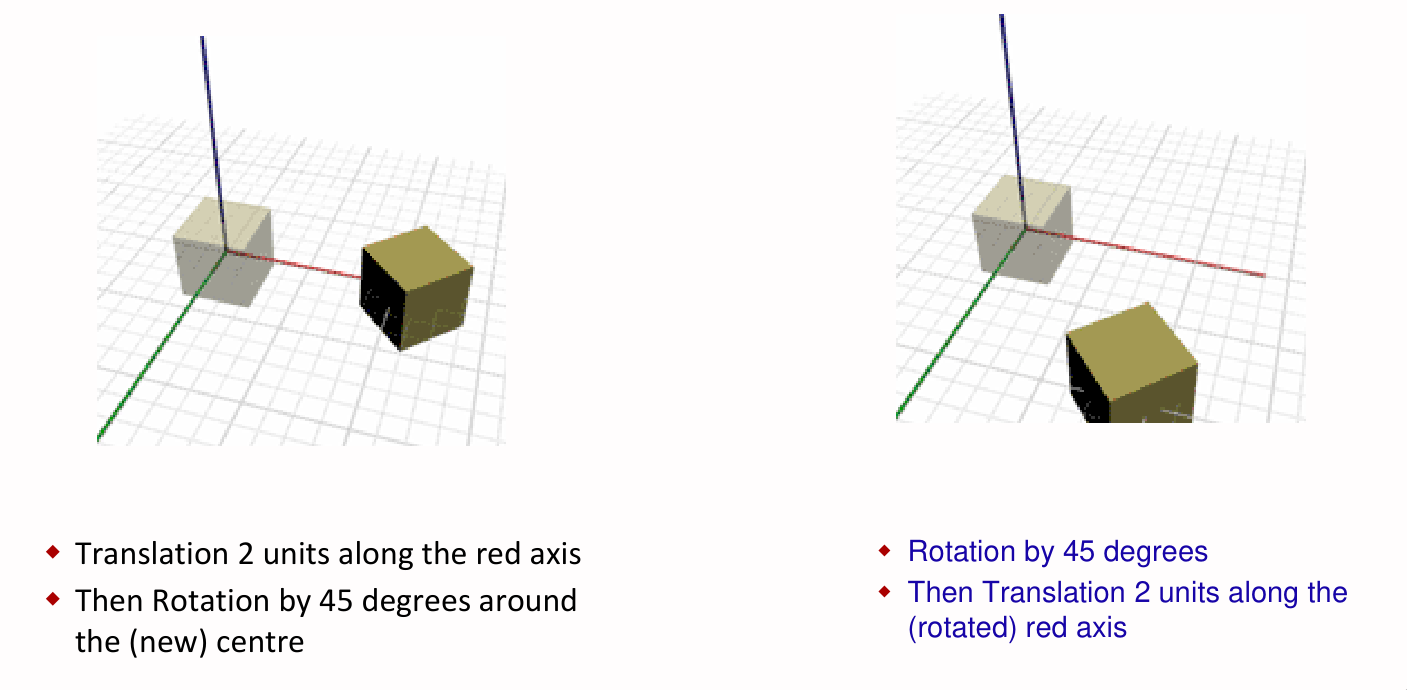
\includegraphics[width=0.8\textwidth]{images/order_of_transformations.png}
    \caption{Order of Transformations}
\end{figure}

\section{2D Raster Graphics}
The raster approach to 2D graphics considers digital images to be grid-based arrays of pixels and operates on the 
images at the pixel level.

\subsection{Introduction to HTML5/Canvas}
\textbf{HTML} or HyperText Markup Language is a page-description language used primarily for website.
\textbf{HTML5} brings major updates \& improvements to the power of client-side web development.
\\\\
A \textbf{canvas} is a 2D raster graphics component in HTML5.
There is also a \textbf{canvas with 3D} (WebGL) which is a 3D graphics component that is more likely to be 
hardware-accelerated but is also more complex.

\subsubsection{Canvas: Rendering Contexts}
\mintinline{html}{<canvas>} creates a fixed-size drawing surface that exposes one or more \textbf{rendering contexts}.
The \mintinline{javascript}{getContext()} method returns an object with tools (methods) for drawing.

\begin{minted}[linenos, breaklines, frame=single]{html}
<html>
    <head>
        <script>
            function draw() {
                var canvas = document.getElementById("canvas");
                var ctx = canvas.getContext("2d");
                ctx.fillStyle = "rgb(200,0,0)";
                ctx.fillRect (10, 10, 55, 50);
                ctx.fillStyle = "rgba(0, 0, 200, 0.5)";
                ctx.fillRect (30, 30, 55, 50);
            }
        </script>
    </head>
    <body onload="draw();">
        <canvas id="canvas" width="150" height="150"></canvas>
    </body>
</html>
\end{minted}

\begin{figure}[H]
    \centering
    
\includegraphics[width=0.2\textwidth]{images/canvas_rendering_contexts.png}
    \caption{Rendering of the Above HTML Code}
\end{figure}

\subsubsection{Canvas2D: Primitives}
Canvas2D only supports one primitive shape: rectangles.
All other shapes must be created by combining one or more \textit{paths}.
Fortunately, there are a collection of path-drawing functions which make it possible to compose complex shapes.

\begin{minted}[linenos, breaklines, frame=single]{javascript}
function draw(){
    var canvas = document.getElementById('canvas');
    var ctx = canvas.getContext('2d');
    ctx.fillRect(125,25,100,100);
    ctx.clearRect(145,45,60,60);
    ctx.strokeRect(150,50,50,50);
    ctx.beginPath();
    ctx.arc(75,75,50,0,Math.PI*2,true); // Outer circle
    ctx.moveTo(110,75);
    ctx.arc(75,75,35,0,Math.PI,false);   // Mouth (clockwise)
    ctx.moveTo(65,65);
    ctx.arc(60,65,5,0,Math.PI*2,true);  // Left eye
    ctx.moveTo(95,65);
    ctx.arc(90,65,5,0,Math.PI*2,true);  // Right eye
    ctx.stroke(); // renders the Path that has been built up..
}
\end{minted}

\begin{figure}[H]
    \centering
    
\includegraphics[width=0.3\textwidth]{images/canvas2d_primitives.png}
    \caption{Rendering of the Above JavaScript Code}
\end{figure}

\subsubsection{Canvas2D: \mintinline{javascript}{drawImage()}}
The example below uses an external image as the backdrop of a small line graph:
\begin{minted}[linenos, breaklines, frame=single]{javascript}
function draw() {
    var ctx = document.getElementById('canvas').getContext('2d');
    var img = new Image();
    img.src = 'backdrop.png';
    img.onload = function(){
        ctx.drawImage(img,0,0);
        ctx.beginPath();
        ctx.moveTo(30,96);
        ctx.lineTo(70,66);
        ctx.lineTo(103,76);
        ctx.lineTo(170,15);
        ctx.stroke();
    }
}
\end{minted}

\begin{figure}[H]
    \centering
    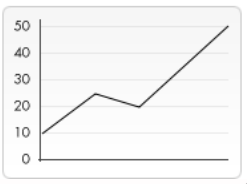
\includegraphics[width=0.3\textwidth]{images/canvas2d_drawimage.png}
    \caption{Rendering of the Above JavaScript Code}
\end{figure}

\subsubsection{Canvas2D: Fill \& Stroke Colours}
\begin{minted}[linenos, breaklines, frame=single]{html}
<html>
    <head>
        <script>
            function draw() {
                var canvas = document.getElementById("canvas");
                var context = canvas.getContext('2d');
                // Filled Star
                context.lineWidth=3;
                context.fillStyle="#CC00FF";
                context.strokeStyle="#ffff00"; // NOT lineStyle!
                context.beginPath();
                context.moveTo(100,50);
                context.lineTo(175,200);
                context.lineTo(0,100);
                context.lineTo(200,100);
                context.lineTo(25,200);
                context.lineTo(100,50);
                context.fill(); // colour the interior
                context.stroke(); // draw the lines
            }
        </script>
    </head>
    <body onload="draw();">
        <canvas id="canvas" width="300" height="300"></canvas>
    </body>
</html>
\end{minted}

Colours can be specified by name (\mintinline{javascript}{red}), by a string of the form
\mintinline{javascript}{rgb(r,g,b)}, or by hexadecimal colour codes \mintinline[escapeinside=||]{javascript}{|#|RRGGBB}.

\begin{figure}[H]
    \centering
    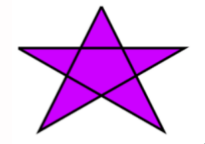
\includegraphics[width=0.3\textwidth]{images/canvas2d_fill_stroke.png}
    \caption{Rendering of the Above JavaScript Code}
\end{figure}

\subsubsection{Canvas2D: Translations}
\begin{minted}[linenos, breaklines, frame=single]{html}
<html>
    <head>
        <script>
            function draw() {
                var canvas = document.getElementById("canvas");
                var context = canvas.getContext('2d');
                context.save(); // save the default (root) co-ord system
                context.fillStyle="#CC00FF"; // purple
                context.fillRect(100,0,100,100);
                // translates from the origin, producing a nested co-ordinate system
                context.translate(75,50);
                context.fillStyle="#FFFF00"; // yellow
                context.fillRect(100,0,100,100);
                // transforms further, to produce another nested co-ordinate system
                context.translate(75,50);
                context.fillStyle="#0000FF"; // blue
                context.fillRect(100,0,100,100);
                context.restore(); // recover the default (root) co-ordinate system
                context.translate(-75,90);
                context.fillStyle="#00FF00"; // green
                context.fillRect(100,0,100,100);
            }
        </script>
    </head>
    <body onload="draw();">
        <canvas id="canvas" width="600" height="600"></canvas>
    </body>
</html>
\end{minted}

\begin{figure}[H]
    \centering
    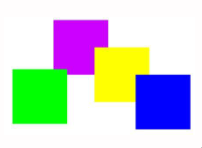
\includegraphics[width=0.3\textwidth]{images/canvas2d_translations.png}
    \caption{Rendering of the Above JavaScript Code}
\end{figure}

\subsubsection{Canvas2D: Order of Transformations}
\begin{minted}[linenos, breaklines, frame=single]{html}
<html>
    <head>
        <script>
            function draw() {
                var canvas = document.getElementById("canvas");
                var context = canvas.getContext('2d');
                context.save(); // save the default (root) co-ord system
                context.fillStyle="#CC00FF"; // purple
                context.fillRect(0,0,100,100); // positioned with TL corner at 0,0
                // translate then rotate
                context.translate(100,0);
                context.rotate(Math.PI/3);
                context.fillStyle="#FF0000"; // red
                context.fillRect(0,0,100,100); // positioned with TL corner at 0,0
                // recover the root co-ord system
                context.restore();
                // rotate then translate
                context.rotate(Math.PI/3);
                context.translate(100,0);
                context.fillStyle="#FFFF00"; // yellow
                context.fillRect(0,0,100,100); // positioned with TL corner at 0,0
            }
        </script>
    </head>
    <body onload="draw();">
        <canvas id="canvas" width="600" height="600"></canvas>
    </body>
</html>
\end{minted}

\begin{figure}[H]
    \centering
    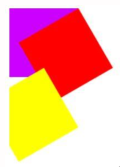
\includegraphics[width=0.2\textwidth]{images/canvas2d_order_of_transformations.png}
    \caption{Rendering of the Above JavaScript Code}
\end{figure}

\subsubsection{Scaling}
\begin{minted}[linenos, breaklines, frame=single]{html}
<html>
    <head>
        <script>
            function draw() {
                var canvas = document.getElementById("canvas");
                var context = canvas.getContext('2d');
                context.fillStyle="#CC00FF"; // purple
                context.fillRect(0,0,100,100); // positioned with TL corner at 0,0
                context.translate(150,0);
                context.scale(2,1.5);
                context.fillStyle="#FF0000"; // red
                context.fillRect(0,0,100,100); // positioned with TL corner at 0,0
            }
        </script>
    </head>
    <body onload="draw();">
        <canvas id="canvas" width="600" height="600"></canvas>
    </body>
</html>
\end{minted}

\begin{figure}[H]
    \centering
    
\includegraphics[width=0.2\textwidth]{images/canvas2d_scaling.png}
    \caption{Rendering of the Above JavaScript Code}
\end{figure}

\subsubsection{Canvas2D: Programmatic Graphics}
\begin{minted}[linenos, breaklines, frame=single]{html}
<html>
    <head>
        <script>
            function draw() {
                var canvas = document.getElementById("canvas");
                var context = canvas.getContext('2d');
                context.translate(150,150);
                for (i=0;i<15;i++) {
                    context.fillStyle = "rgb("+(i*255/15)+",0,0)";
                    context.fillRect(0,0,100,100);
                    context.rotate(2*Math.PI/15);
                }
            }
        </script>
    </head>
    <body onload="draw();">
        <canvas id="canvas" width="600" height="600"></canvas>
    </body>
</html>
\end{minted}

\begin{figure}[H]
    \centering
    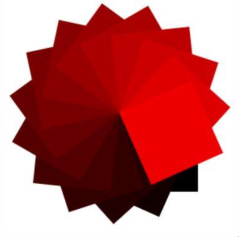
\includegraphics[width=0.2\textwidth]{images/canvas2d_programmatic_graphics.png}
    \caption{Rendering of the Above JavaScript Code}
\end{figure}

\section{3D Co-Ordinate Systems}
In a 3D co-ordinate system, a point $P$ is referred to by three real numbers (co-ordinates): $(x,y,z)$.
The directions of $x$, $y$, \& $z$ are not universally defined but normally follow the \textbf{right-hand rule}
for axes systems.
In this case, $z$ defined the co-ordinate's distance ``out of'' the monitor and negative $z$ values go ``into''
the monitor.

\subsection{Nested Co-Ordinate Systems}
A \textbf{nested co-ordinate system} is defined as a translation relative to the world co-ordinate system.
For example, $-3.0$ units along the $x$ axis, $2.0$ units along the $y$ axis, and $2.0$ units along the $z$ axis.

\subsection{3D Transformations}
\subsubsection{Translation}
To translate a 3D point, modify each dimension separately:
$$
x' = x + a_1
$$
$$
y' = y + a_2
$$
$$
z' = z + a_3
$$

$$
\begin{bmatrix}
    x' & y' & z' & 1
\end{bmatrix}
=
\begin{bmatrix}
    x & y & z & 1
\end{bmatrix}
\begin{bmatrix}
    1   & 0 & 0 & 0 \\
    0   & 1 & 0 & 0 \\
    0   & 0 & 1 & 0 \\
    a_1 & a_2 & a_3 & 1
\end{bmatrix}
$$

\subsubsection{Rotation About Principal Axes}
A \textbf{principal axis} is an imaginary line through the ``center of mass'' of a body around which the body 
rotates.
\begin{itemize}
    \item   Rotation around the $x$-axis is referred to as \textbf{pitch}.
    \item   Rotation around the $y$-axis is referred to as \textbf{yaw}.
    \item   Rotation around the $z$-axis is referred to as \textbf{roll}.
\end{itemize}

\textbf{Rotation matrices} define rotations by angle $\alpha$ about the principal axes.
$$
R_x =
\begin{bmatrix}
    1 & 0 & 0 \\
    0 & \cos \alpha & \sin \alpha \\
    0 & - \sin \alpha & \cos \alpha
\end{bmatrix}
$$

To get new co-ordinates after rotation, multiply the point $\begin{bmatrix} x & y & z \end{bmatrix}$ by the
rotation matrix:
$$
\begin{bmatrix}
    x' & y' & z'
\end{bmatrix}
=
\begin{bmatrix}
    x & y & z
\end{bmatrix}
R_x
$$

For example, as a point rotates about the $x$-axis, its $x$ component remains unchanged.

\subsubsection{Rotation About Arbitrary Axes}
You can rotate about any axis, not just the principal axes.
You specify a 3D point, and the axis of rotation is defined as the line that joins the origin to this point
(e.g., a toy spinning top will rotate about the $y$-axis, defined as $(0, 1, 0)$).
You must also specify the amount to rotate by, this is measured in radians (e.g., $2\pi$ radians is $360\degree$).

\section{Graphics APIs}
\textbf{Low-level} graphics APIs are libraries of graphics functions that can be accessed from a standard 
programming language.
They are typically procedural rather than descriptive, i.e. the programmer calls the graphics functions which 
carry out operations immediately.
The programmer also has to write all other application code: interface, etc.
Procedural programming languages are typically faster than descriptive programming languages.
Examples include OpenGL, DirectX, Vulkan, Java Media APIs.
Examples that run in the browser include Canvas2D, WebGL, SVG.
\\\\
\textbf{High-level} graphics APIs are ones in which the programmer describes the required graphics, animations,
interactivity, etc. and doesn't need to deal with how this will be displayed \& updated.
They are typically descriptive rather than procedural and so are generally slower \& less flexible because it is 
generally interpreted and rather general-purpose rather than task-specific.
Examples include VRML/X3D.

\subsection{Three.js}
\textbf{WebGL (Web Graphics Library)} is a JavaScript API for rendering interactive 2D \& 3D graphics within any
compatible web browser without the use of plug-ins.
WebGL s fully integrated with other web standards, allowing GPU-accelerated usage of physics \& image processing
and effects as part of the web page canvas.
\\\\
\textbf{Three.js} is a cross-browser JavaScript library and API used to create \& display animated 4D computer 
graphics in a web browser.
Three.js uses WebGL.

\begin{code}
\begin{minted}[linenos, breaklines, frame=single]{html}
<html>
 <head>
  
  <script src="three.js"></script>
  <script>
    'use strict'

    function draw() {
      // create renderer attached to HTML Canvas object
      var c = document.getElementById("canvas");
      var renderer = new THREE.WebGLRenderer({ canvas: c, antialias: true });

      // create the scenegraph
      var scene = new THREE.Scene();

      // create a camera
      var fov = 75;
      var aspect = 600/600;
      var near = 0.1;
      var far = 1000;
      var camera = new THREE.PerspectiveCamera( fov, aspect, near, far );
      camera.position.z = 100;

      // add a light to the scene
      var light = new THREE.PointLight(0xFFFF00);
      light.position.set(10, 30, 25);
      scene.add(light);

      // add a cube to the scene
      var geometry = new THREE.BoxGeometry(20, 20, 20);
      var material = new THREE.MeshLambertMaterial({color: 0xfd59d7});
      var cube = new THREE.Mesh(geometry, material);
      scene.add(cube);

      // render the scene as seen by the camera
      renderer.render(scene, camera);
    }
  </script>
 </head>

 <body onload="draw();">
   <canvas id="canvas" width="600" height="600"></canvas>
 </body>
</html>
\end{minted}
\caption{``Hello World'' in Three.js}
\end{code}

In Three.js, a visible object is represented as a \textbf{mesh} and is constructed from a \textit{geometry} \& a
\textit{material}.

\subsubsection{3D Primitives}
Three.js provides a range of primitive geometry as well as the functionality to implement more complex geometry at a lower 
level.
See \url{https://threejs.org/manual/?q=prim#en/primitives}.

\begin{code}
\begin{minted}[linenos, breaklines, frame=single]{html}
<html>
 <head>
  
  <script src="three.js"></script>
  <script>
    'use strict'

    var scene;

    function addGeometryAtPosition(geometry, x, y, z) {
      var material = new THREE.MeshLambertMaterial({color: 0xffffff});
      var mesh = new THREE.Mesh(geometry, material);
      scene.add(mesh);
      mesh.position.set(x,y,z);
    }

    function draw() {
      // create renderer attached to HTML Canvas object
      var c = document.getElementById("canvas");
      var renderer = new THREE.WebGLRenderer({ canvas: c, antialias: true });

      // create the scenegraph (global variable)
      scene = new THREE.Scene();

      // create a camera
      var fov = 75;
      var aspect = 400/600;
      var near = 0.1;
      var far = 1000;
      var camera = new THREE.PerspectiveCamera( fov, aspect, near, far );
      camera.position.z = 100;

      // add a light to the scene
      var light = new THREE.PointLight(0xFFFF00);
      light.position.set(10, 0, 25);
      scene.add(light);

      // add a bunch of sample primitives to the scene
      // see more here:  https://threejsfundamentals.org/threejs/lessons/threejs-primitives.html 

      // args: width, height, depth
      addGeometryAtPosition(new THREE.BoxGeometry(6,4,8), -50, 0, 0);

      // args: radius, segments
      addGeometryAtPosition(new THREE.CircleBufferGeometry(7, 24), -30, 0, 0);

      // args: radius, height, segments
      addGeometryAtPosition(new THREE.ConeBufferGeometry(6, 4, 24), -10, 0, 0);

      // args: radiusTop, radiusBottom, height, radialSegments
      addGeometryAtPosition(new THREE.CylinderBufferGeometry(4, 4, 8, 12), 20, 0, 0);

      // arg: radius 
      // Polyhedrons
      // (Dodecahedron is a 12-sided polyhedron, Icosahedron is 20-sided, Octahedron is 8-sided, Tetrahedron is 4-sided)
      addGeometryAtPosition(new THREE.DodecahedronBufferGeometry(7), 40, 0, 0);
      addGeometryAtPosition(new THREE.IcosahedronBufferGeometry(7), -50, 20, 0);
      addGeometryAtPosition(new THREE.OctahedronBufferGeometry(7), -30, 20, 0);
      addGeometryAtPosition(new THREE.TetrahedronBufferGeometry(7), -10, 20, 0);

      // args: radius, widthSegments, heightSegments
      addGeometryAtPosition(new THREE.SphereBufferGeometry(7,12,8), 20, 20, 0);
      
      // args: radius, tubeRadius, radialSegments, tubularSegments
      addGeometryAtPosition(new THREE.TorusBufferGeometry(5,2,8,24), 40, 20, 0);
      
      // render the scene as seen by the camera
      renderer.render(scene, camera);
    }
  </script>
 </head>

 <body onload="draw();">
   <canvas id="canvas" width="600" height="600"></canvas>
 </body>
</html>
\end{minted}
\caption{Code Illustrating Some Primitives Provided by Three.js}
\end{code}

\subsubsection{Cameras}
3D graphics API cameras allow you to define:
\begin{itemize}
    \item   The camera location $(x,y,z)$.
    \item   The camera orientation (\sout{straight, gay} $x$ rotation, $y$ rotation, $z$ rotation).
    \item   The \textbf{viewing frustum} (the Field of View (FoV) \& clipping planes).
            \begin{figure}[H]
                \centering
                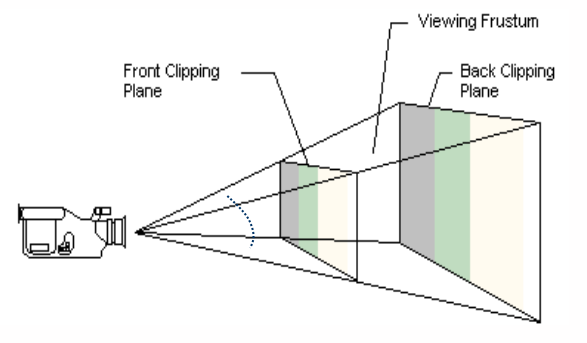
\includegraphics[width=0.5\textwidth]{images/viewing_frustum.png}
                \caption{The Viewing Frustum}
            \end{figure}
\end{itemize}

In Three.js, the FoV can be set differently in the vertical and horizontal directions via the first \& second arguments
to the constructor can be set differently in the vertical and horizontal directions via the first \& second arguments
to the constructor \mintinline{javascript}{(fov, aspect)}.
Generally speaking, the aspect ratio should match that of the canvas width \& height to avoid the scene appearing to be
stretched.

\subsubsection{Lighting}
Six different types of lights are available in both Three.js \& WebGL:
\begin{itemize}
    \item   \textbf{Point lights:} rays emanate in all directions from a 3D point source (e.g., a lightbulb).
    \item   \textbf{Directional lights:} rays emanate in one direction only from infinitely far away
            (similar effect rays from the Sun, i.e. very far away).
    \item   \textbf{Spotlights:} project a cone of light from a 3D point source aimed at a specific target point.
    \item   \textbf{Ambient lights:} simulate in a simplified way the lighting of an entire scene due to complex 
            light/surface interactions -- lights up everything in the scene regardless of position or occlusion.
    \item   \textbf{Hemisphere lights:} ambient lights that affect the ``ceiling'' or ``floor'' hemisphere of objects
            rather than affecting them in their entirety.
    \item   \textbf{RectAreaLights:} emit rectangular areas of light (e.g., fluorescent light strip).
\end{itemize}

\begin{code}
\begin{minted}[linenos, breaklines, frame=single]{html}
<html>
  <head>
  <script src="three.js"></script>
  <script>
    'use strict'

    function draw() {
      // create renderer attached to HTML Canvas object
      var c = document.getElementById("canvas");
      var renderer = new THREE.WebGLRenderer({ canvas: c, antialias: true });

      // create the scenegraph
      var scene = new THREE.Scene();

      // create a camera
      var fov = 75;
      var aspect = 600/600;
      var near = 0.1;
      var far = 1000;
      var camera = new THREE.PerspectiveCamera( fov, aspect, near, far );
      camera.position.set(0, 10, 30);

      // add a light to the scene
      var light = new THREE.PointLight(0xFFFFFF);
      light.position.set(0, 10, 30);
      scene.add(light);

      // add a cylinder 
      // args: radiusTop, radiusBottom, height, radialSegments
      var cyl = new THREE.Mesh(
        new THREE.CylinderBufferGeometry(1, 1, 10, 12), 
        new THREE.MeshLambertMaterial({color: 0xAAAAAA}) );
      scene.add(cyl);

      // clone the cylinder
      var cyl2 = cyl.clone();
     
      // modify its rotation by 60 degrees around its z axis
      cyl2.rotateOnAxis(new THREE.Vector3(0,0,1), Math.PI/3);
      scene.add(cyl2);
      // clone the cylinder again
      var cyl3 = cyl.clone();
      scene.add(cyl3);
      // set its rotation directly using "Euler angles", to 120 degrees on z axis
      cyl3.rotation.set(0,0,2*Math.PI/3);
      
      // render the scene as seen by the camera
      renderer.render(scene, camera);
    }
  </script>
 </head>

 <body onload="draw();">
   <canvas id="canvas" width="600" height="600"></canvas>
 </body>
</html>
\end{minted}
\caption{Rotation Around a Local Origin in Three.js}
\end{code}

\subsubsection{Nested Co-Ordinates}
\textbf{Nested co-ordinates} help manage complexity as well as promote reusability \& simplify the transformations of
objects composed of multiple primitive shapes.
In Three.js, 3D objects have a \mintinline{javascript}{children} array;
a child can be added to an object using the method \mintinline{javascript}{.add(childObject)}, i.e. nesting the child 
object's transform within the parent object.
Objects have a parent in the scene graph so when you set their transforms (translation, rotation) it's relative to that
parent's local co-ordinate system.


\begin{code}
\begin{minted}[linenos, breaklines, frame=single]{html}
<html>
 <head>
  
  <script src="three.js"></script>
  <script>
    'use strict'

    function draw() {
      // create renderer attached to HTML Canvas object
      var c = document.getElementById("canvas");
      var renderer = new THREE.WebGLRenderer({ canvas: c, antialias: true });

      // create the scenegraph 
      var scene = new THREE.Scene();

      // create a camera
      var fov = 75;
      var aspect = 600/600;
      var near = 0.1;
      var far = 1000;
      var camera = new THREE.PerspectiveCamera( fov, aspect, near, far );
      camera.position.set(0, 1.5, 6);

      // add a light to the scene
      var light = new THREE.PointLight(0xFFFFFF);
      light.position.set(0, 10, 30);
      scene.add(light);

      // desk lamp base
      // args: radiusTop, radiusBottom, height, radialSegments
      var base = new THREE.Mesh(
        new THREE.CylinderBufferGeometry(1, 1, 0.1, 12), 
        new THREE.MeshLambertMaterial({color: 0xAAAAAA}) );
      scene.add(base);

      // desk lamp first arm piece
      var arm = new THREE.Mesh(
        new THREE.CylinderBufferGeometry(0.1, 0.1, 3, 12), 
        new THREE.MeshLambertMaterial({color: 0xAAAAAA}) );

      // since we want to rotate around a point other than the arm's centre,
      // we can create a pivot point as the parent of the arm, position the
      // arm relative to that pivot point, and apply rotation on the pivot point
      var pivot = new THREE.Object3D();
      // centre of rotation we want 
      // (in world coordinates, since pivot is not yet a child of the base)
      pivot.position.set(0, 0, 0); 
      pivot.add(arm); // pivot is parent of arm
      base.add(pivot); // base is parent of pivot

      //  translate arm relative to its parent, i.e. 'pivot'
      arm.position.set(0, 1.5, 0);
      //  rotate pivot point relative to its parent, i.e. 'base'
      pivot.rotateOnAxis(new THREE.Vector3(0,0,1), -Math.PI/6);

      // clone a second arm piece (consisting of a pivot with a cylinder as its child)
      var pivot2 = pivot.clone();
      // add as a child of the 1st pivot
      pivot.add(pivot2);
      // rotate the 2nd pivot relative to the 1st pivot (since it's nested)
      pivot2.rotation.z = Math.PI/3;
      // translate the 2nd pivot relative to the 1st pivot
      pivot2.position.set(0,3,0);

      // TEST: we can rotate the 1st arm piece and the 2nd arm piece should stay correct
      pivot.rotateOnAxis(new THREE.Vector3(0,0,1), Math.PI/12);

      // TEST: we can also move the base, and everything stays correct
      base.position.x -= 3;
      
      // render the scene as seen by the camera
      renderer.render(scene, camera);
    }
  </script>
 </head>

 <body onload="draw();">
   <canvas id="canvas" width="600" height="600"></canvas>
 </body>
</html>
\end{minted}
\caption{Partial Desk Lamp with Nested Objects}
\end{code}

The above code creates a correctly set-up hierarchy of nested objects, allowing us to:
\begin{itemize}
    \item   Translate the base while the two arms remain in the correct relative position.
    \item   Rotate the first arm while keeping the second arm in the correct position.
\end{itemize}

\subsubsection{Geometry Beyond Primitives}
In Three.js, the term ``low-level geometry'' is used to refer to geometry objects consisting of vertices, faces, \& 
normal.

\section{Animation \& Interactivity}
\subsection{Handling the Keyboard}
Handling the keyboard involves recognising keypresses and updating the graphics in response.

\begin{code}
    \inputminted[linenos, breaklines, frame=single]{html}{../materials/week3/examples/canvasWithKeyboardExample.html}
    \caption{Keyboard Handling (Canvas/JavaScript)}
\end{code}

\subsection{Mouse Handling}
\begin{code}
    \inputminted[linenos, breaklines, frame=single]{html}{../materials/week3/examples/canvasWithMouseExample.html}
    \caption{Mouse Handling (Canvas/JavaScript)}
\end{code}

\subsection{Time-Based Animation}
Time-based animation can be achieved using \mintinline{javascript}{window.setTimeout()} which repaints the 
canvas at pre-defined intervals.

\begin{code}
    \inputminted[linenos, breaklines, frame=single]{html}{../materials/week3/examples/canvasAnimationExample1.html}
    \caption{Time-Based Animation with \mintinline{javascript}{window.setTimeout()}}
\end{code}

However, improved smoothness can be achieved using \mintinline{javascript}{window.requestAnimationFrame()} which is called at
every window repaint/refresh.

\begin{code}
    \inputminted[linenos, breaklines, frame=single]{html}{../materials/week3/examples/canvasAnimationExample1_withSmootherAnimation.html}
    \caption{Smoother Time-Based Animation with \mintinline{javascript}{window.requestAnimationFrame()}}
\end{code}

\subsection{Raycasting}
\textbf{Raycasting} is a feature offered by 3D graphics APIs which computes a ray from a start position in a specified direction
and identifies the geometry that the ray hits.
\begin{minted}[linenos, breaklines, frame=single]{html}
renderer = new THREE.WebGLRenderer({ canvas: c, antialias: true });
\end{minted}

The following example illustrates the use of raycasting/picking and rotation/translation based on mouse selection and mouse 
movement.
It also illustrates how nested co-ordinate systems have been used to make the lamp parts behave correctly.

\begin{code}
    \inputminted[linenos, breaklines, frame=single]{html}{../materials/week3/examples/Threejs-20-controllable-desk-lamp.html}
    \caption{Controllable Desk Lamp}
\end{code}

\subsection{Shading Algorithms}
The colour at any pixel on a polygon is determined by:
\begin{itemize}
    \item   The characteristics (including colour) of the surface itself.
    \item   Information about light sources (ambient, directional, parallel, point, or spot) and their positions relative to
            the surface.
    \item   \textit{Diffuse} \& \textit{specular} reflections.
\end{itemize}

Classic shading algorithms include:
\begin{itemize}
    \item   Flat shading.
    \item   Smooth shading (Gourard).
    \item   Normal Interpolating Shading (Phong).
\end{itemize}

\begin{figure}[H]
    \centering
    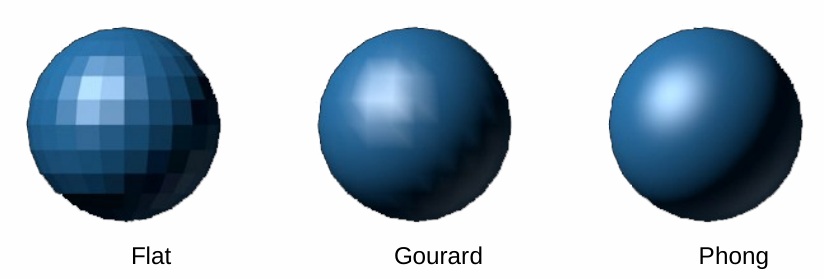
\includegraphics[width=\textwidth]{images/shading_algs.png}
    \caption{Different Shading Algorithms}
\end{figure}

\subsubsection{Flat Shading}
\textbf{Flat shading} calculates and applies directly the shade of each surface, which is calculated via the cosine of the angle
of incidence ray to the \textit{surface normal} (a \textbf{surface normal} is a vector perpendicular to the surface).

\begin{figure}[H]
    \centering
    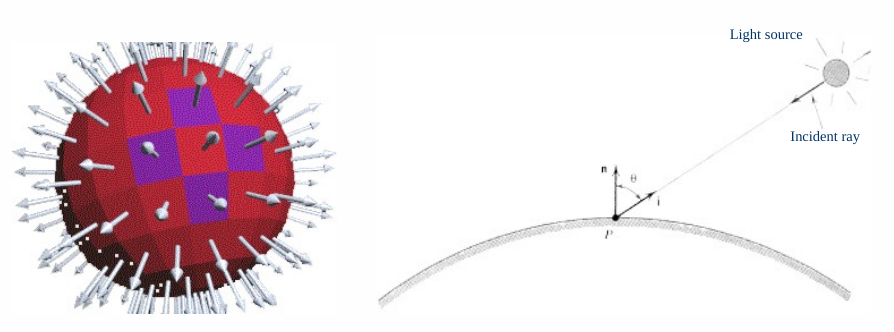
\includegraphics[width=\textwidth]{images/flat_shading.png}
    \caption{Flat Shading}
\end{figure}

\subsubsection{Smooth (Gourard) Shading}
\textbf{Smooth (Gourard) shading} calculates the shade at each vertex, and interpolates (smooths) these shades across the 
surfaces.
Vertex normals are calculated by averaging the normals of the connected faces.
Interpolation is often carried out in graphics hardware, making it generally very fast.

\begin{figure}[H]
    \centering
    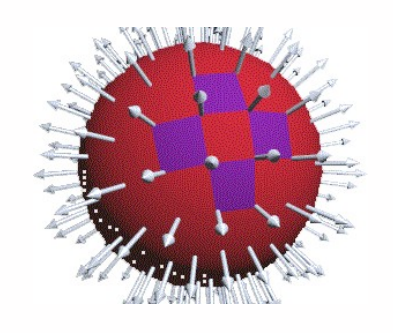
\includegraphics[width=0.5\textwidth]{images/smooth_shading.png}
    \caption{Smooth Shading}
\end{figure}

\subsubsection{Normal Interpolating (Phong) Shading}
\textbf{Normal interpolating (Phong) shading} calculates the normal at each vertex and interpolates these normals across the
surfaces.
The light, and therefore the shade at each pixel is individually calculated from its unique surface normal.

\begin{figure}[H]
    \centering
    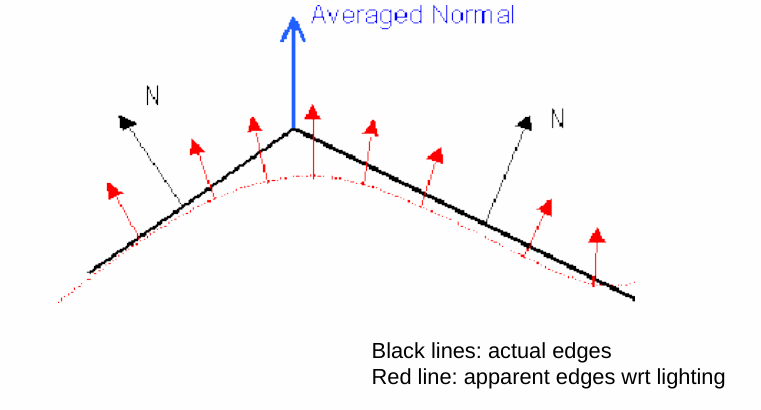
\includegraphics[width=0.5\textwidth]{images/phong_shading.png}
    \caption{Normal Interpolating (Phong) Shading}
\end{figure}

\subsection{Shading in Three.js}
In Three.js, \textbf{materials} define how objects will be shaded in the scene.
There are three different shading models to choose from:
\begin{itemize}
    \item   \mintinline{javascript}{MeshBasicMaterial}: none.
    \item   \mintinline{javascript}{MeshPhongMaterial} (with \mintinline{javascript}{flatShading = true}): flat shading.
    \item   \mintinline{javascript}{MeshLamberMaterial}: Gourard shading.
\end{itemize}

\subsection{Shadows in Three.js}
Three.js supports the use of shadows although they are expensive to use.
The scene is redrawn for each shadow-casting light, and finally composed from all the results.
Games sometimes use fake ``blob shadows'' instead of proper shadows or else only let one light cast shadows to save computation.

\subsection{Reflectivity of Materials in Three.js}
There are a variety of colour settings in Three.js
\begin{itemize}
    \item   \textbf{Diffuse colour} is defined by the colour of the material.
    \item   \textbf{Specular colour} is the colour of specular highlights (in Phong shading only).
    \item   \textbf{Shininess} is the strength of specular highlights (in Phong only).
    \item   \textbf{Emissive colour} is not affected by lighting.
\end{itemize}

\section{Image Processing}
The difference between Graphics, Image Processing, \& Computer Vision is as follows:
\begin{itemize}
    \item   \textbf{Graphics} is the processing \& display of images of objects that exist conceptually rather than physically, wit emphasis on the generation of an image from a model of the objects, illumination, etc. and an emphasis on the rendering efficiency for real-time display and/or realism.

    \item   \textbf{Image Processing} is the processing \& analysis of images of the real world, with an emphasis on the modification of the image.

    \item   \textbf{Computer Vision} uses image processing, techniques from AI, \& pattern recognition to recognise \& categorise image data and extract domain-specific information from these images.
\end{itemize}

Image processing techniques include:
\begin{itemize}
    \item   \textbf{Image Enhancement:} provide a more effective display of data for visual interpretation or increase the visual distinction between features in the image.
    \item   \textbf{Image Restoration:} correction of geometrics distortions, de-noising, de-blurring, etc.
    \item   \textbf{Feature Extraction:} the extraction of useful features, e.g. corners, blobs, edges, \& lines, the extraction of image segments \& regions of interest, and the subtraction of background to extract foreground objects.
\end{itemize}

Image processing applications include industrial inspection, document image analysis, traffic monitoring, security and surveillance, remote sensing, scientific imaging, medical imaging, robotics and autonomous systems, face analysis and biometric, \& entertainment  

\subsection{Introduction to OpenCV}
\textbf{Open Source Computer Vision Library (OpenCV)} is an open source computer vision \& machine learning software library which is available for Python, C++, JavaScript, \& Java.
It is a good choice for high-performance image processing and for making use of pre-built library functions.
\\\\
You can also write image processing code directly using Canvas \& JavaScript or Matlab Image Processing \& Computer Vision toolboxes.

\subsection{Point Transformations}
\textbf{Point transformations} modify the value of each pixel.

\subsubsection{Histogram Manipulation}
A \textbf{histogram} is a graphical representation of the distribution of pixel intensity values in an image.
It displays the number of pixels for each intensity level, allowing us to understand the image's overall brightness \& contrast.
Histogram manipulation utilises the following processes:
\begin{itemize}
    \item   \textbf{Contrast Stretching:} enhancing the contrast of an image by spreading out the intensity values across the available range, with the goal of making the distinction between different pixel values more apparent.
            \textbf{Uniform expansion / linear stretch} is a method of contrast stretching that assigns a proportional number of grey levels to both frequently \& rarely occurring pixel values.
            It aims to ensure that every pixel intensity has a chance to occupy the full range of values, and can be applied either globally (to the entire image) or locally (to smaller regions).

            \begin{minipage}{\linewidth}
                \begin{figure}[H]
                    \centering
                    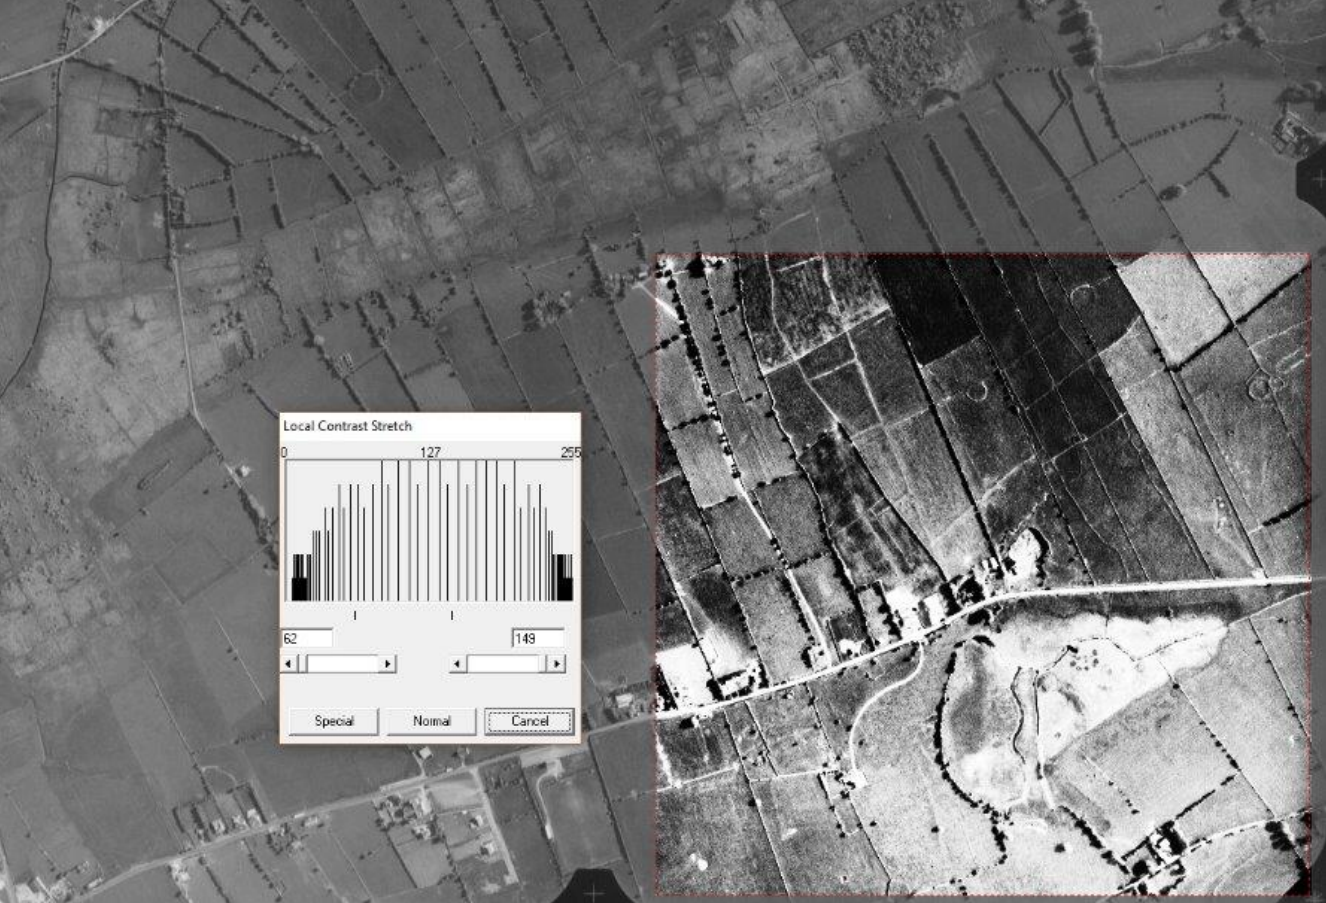
\includegraphics[width=\linewidth]{images/local_histogram_stretch_aerial.png}
                    \caption{Aerial Photograph with a Local Histogram Stretch Applied}
                \end{figure}
            \end{minipage}

    \item   \textbf{Histogram Equalisation} is a process that adjusts the intensity distribution of an image to achieve a uniform histogram.
            It enhances contrast by redistributing pixel values, which helps in revealing more details, particularly in images where some pixel values are too dominant or too rare.

            \begin{minipage}{\linewidth}
                \begin{figure}[H]
                    \centering
                    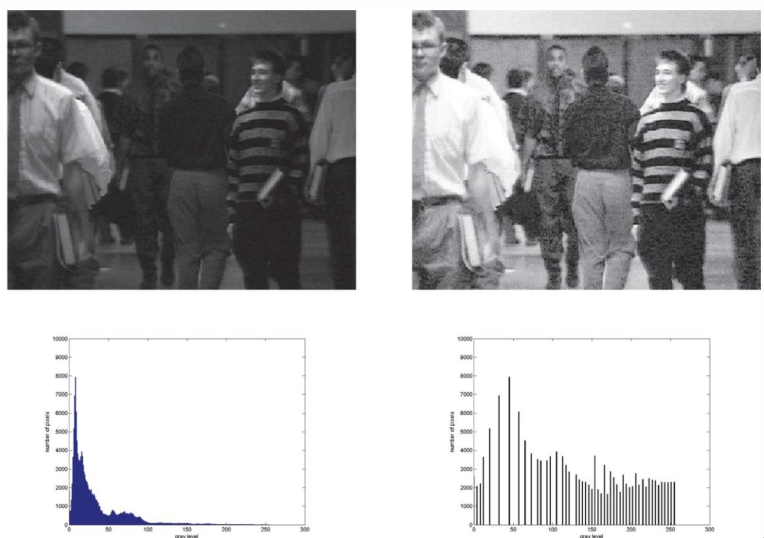
\includegraphics[width=\linewidth]{images/hoop_dreams.png}
                    \caption{Histogram Equalisation Applied with Discretisation Effects}
                \end{figure}
            \end{minipage}
\end{itemize}

\subsubsection{Thresholding}
\textbf{Thresholding} is a simple segmentation technique that is very useful for separating solid objects from a contrasting background.
All pixels above a determined threshold grey level are assumed to belong to the object, and all pixels below that level are assumed to be outside that object (or vice-versa).
The selection of the threshold level is very important: problems of over-segmentation exist (false negatives) and under-segmentation (false positives).

\begin{figure}[H]
    \centering
    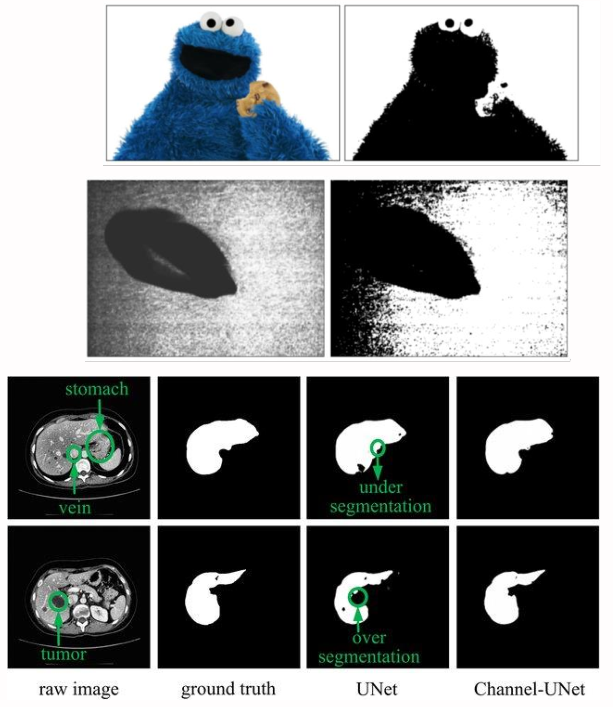
\includegraphics[width=0.44\textwidth]{images/thresholding_examples.png}
    \caption{Thresholding Examples}
\end{figure}

\subsection{Geometric Transformations}
\subsubsection{Interpolation}
As a 2D arrray of values, a digital image can be thought of as a sampling of an underlying continuous function.
Interpolation estimates this underlying continuous function by computing pixel values at real-valued co-ordinates where the estimated continuous function must coincide with the sampled data at the sample points.
Types of interpolation include:
\begin{itemize}
    \item   Nearest-neighbour interpolation.
    \item   Bilinear interpreation which calculates a distance-weighted average of the four pixels closest to the target sub-pixel position $(v,w)$.
    \item   Bicubic interpolation which is more accurate but costly, where derivatives of the underlying function are also estimated.
\end{itemize}

\begin{figure}[H]
    \centering
    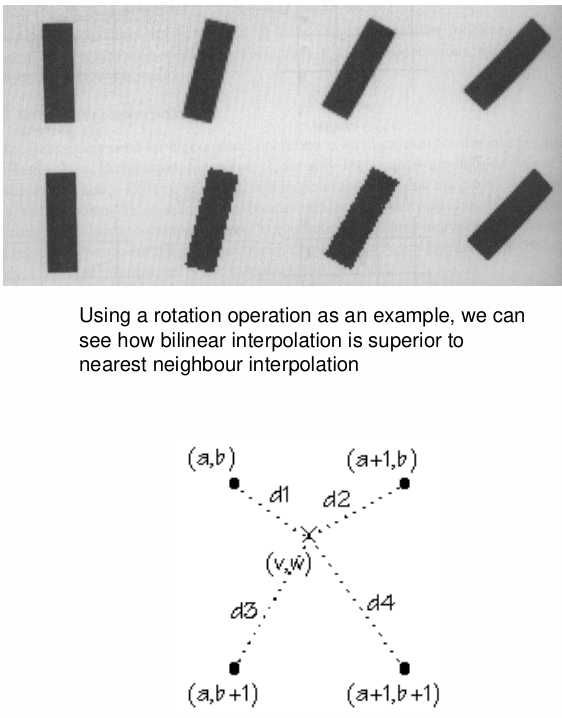
\includegraphics[width=0.5\textwidth]{images/interpolation_examples.png}
    \caption{Interpolation Examples}
\end{figure}

\subsubsection{Warping}
\textbf{Warping} consists of arbitrary geometric transformations from real-valued co-ordinates $(x,y)$ to real-valued co-ordinates $(x^\prime, y^\prime)$ where the mapping function $f(x,y)$ specifies the transformation, or \textit{warping}.
Applications include image rectification, image registration, map projection, \& image morphing.

\begin{figure}[H]
    \centering
    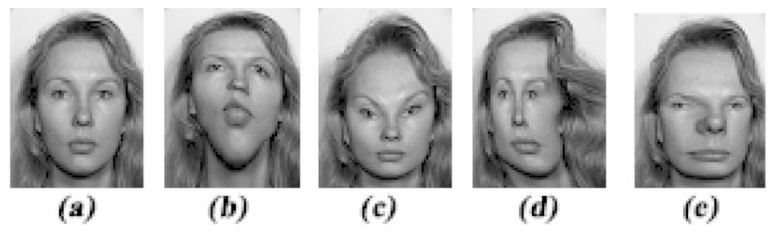
\includegraphics[width=0.5\textwidth]{images/warping_examples.png}
    \caption{Warping Examples}
\end{figure}

\subsubsection{Image Rectification}
\textbf{Image rectification} (part of camera calibration) is a standard approach to geometric correction consisting of displacement values for specified control points in the image.
Displacement of non-control points is determined through \textit{interpolation}.
For example, take a photograph of a rectangular grid and then determine the mapping required to move output control points back to known undistorted positions.

\begin{figure}[H]
    \centering
    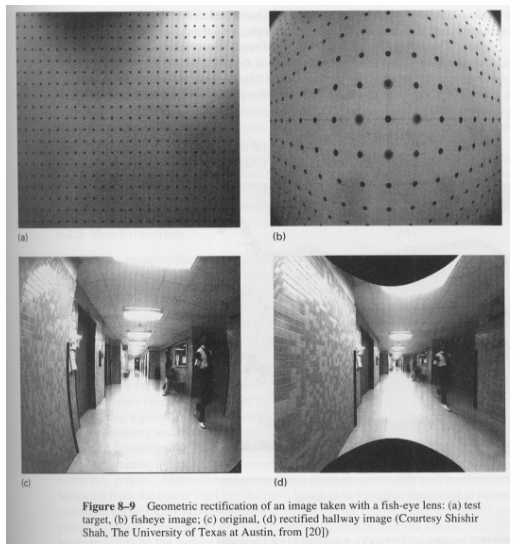
\includegraphics[width=0.5\textwidth]{images/rectification_examples.png}
    \caption{Image Rectification Examples}
\end{figure}

\subsubsection{Image Registration}
\textbf{Image registration} is the process of transforming different sets of data into one co-ordinate system.
Geometric operations are applied to images for the purposes of comparison, monitoring, measurement, etc. and have many applications in medical imaging.

\begin{figure}[H]
    \centering
    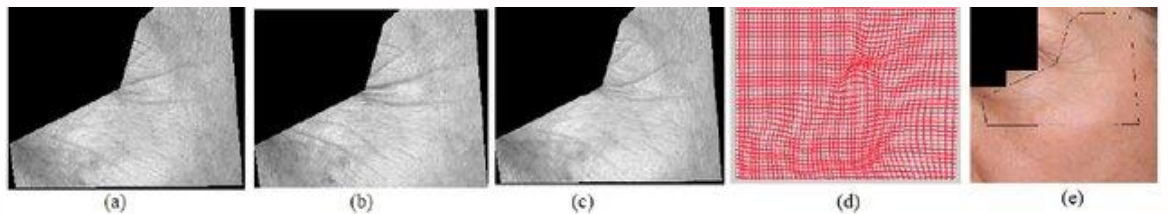
\includegraphics[width=\textwidth]{images/image_registration.png}
    \caption{Image Registration Examples}
\end{figure}

\subsubsection{Map Projection}
Aerial or spaceborne images of the surface of a planet may be rectified into photomaps.
Both oblique and orthoganol photographs require correction for this application due to the shape of the surface being imaged.

\begin{figure}[H]
    \centering
    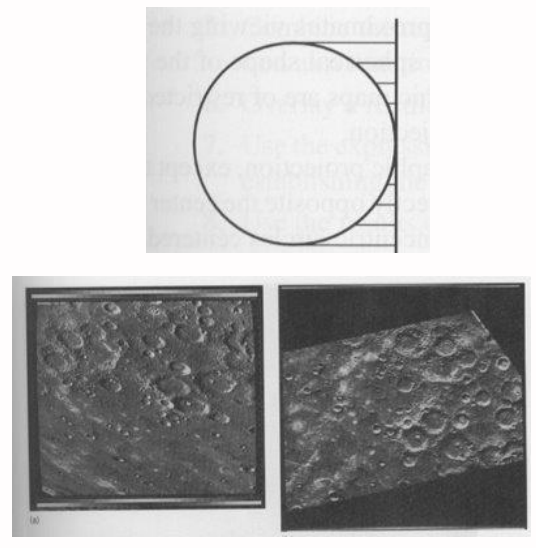
\includegraphics[width=0.5\textwidth]{images/map_projection.png}
    \caption{Map Projection Examples}
\end{figure}

\subsubsection{Image Morphing}
\textbf{Image morphing} gradually transforms one image into another over a number of animation frames.
It involves a dissolve from one image to the other (i.e., gradual change of pixel values) as well as an incremental geometric operation using control points (e.g., nostrils, eyes, chin, etc.).

\begin{figure}[H]
    \centering
    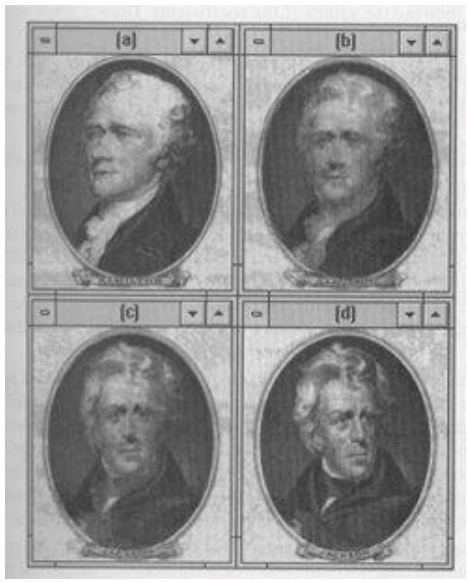
\includegraphics[width=0.5\textwidth]{images/image_morphing.png}
    \caption{Image Morphing Examples}
\end{figure}

\section{Spatial Filtering}
Spatial filtering is a fundamental local operation in image processing that is used for a variety of tasks, including noise removal, blurring, sharpening, \& edge detection.
It establishes a moving window called a \textbf{kernel} which contains an array of coefficients or weighting factors.
The kernel is then moved across the original image so that it centres on each pixel in turn.
Each coefficient in the kernel is multiplied by the value of the pixel below it, and the addition of each of these values determines the value of the pixel in the output image corresponding to the pixel in the centre of the kernel. 
\begin{itemize}
    \item   \textbf{Smoothing kernels} perform an averaging of the values in a local neighbourhood and therefore reduce the effects of noise.
            Such kernels are often used as the first stage of pre-processing an image that has been corrupted by noise in order to restore the original image.
    \item   \textbf{Differentiating kernels} accentuate the places where the signal is changing in value rapidly.
            They are used to extract useful information from images, such as the boundaries of objects, for purposes such as object detection.
\end{itemize}

\begin{figure}[H]
    \centering
    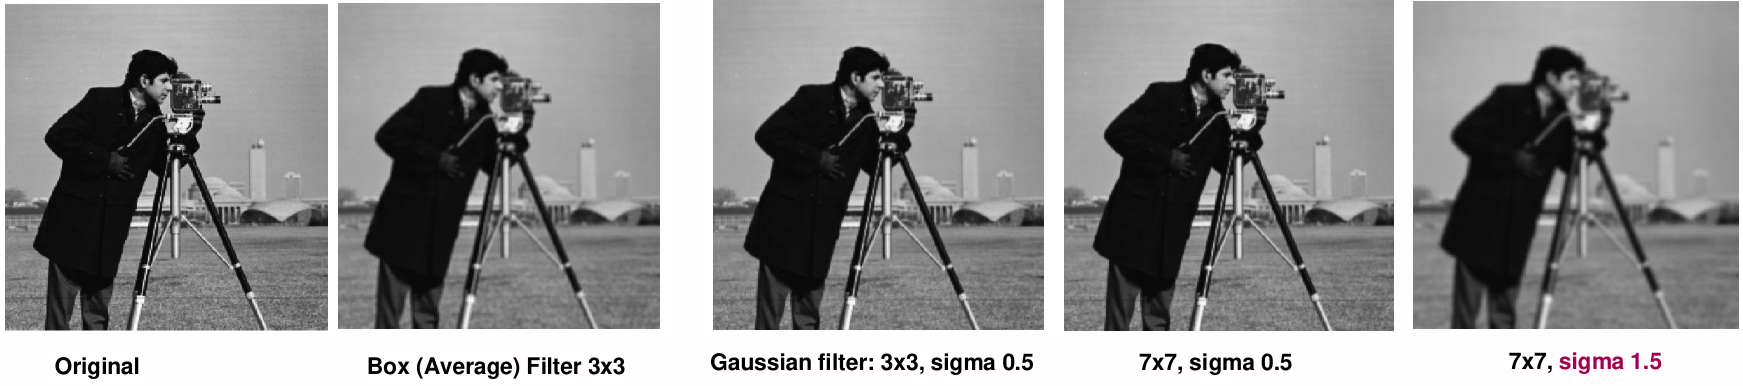
\includegraphics[width=\textwidth]{images/spatial_filtering_smoothing_filters.png}
    \caption{Spatial Filtering: Smoothing Filters}
\end{figure}

For symmetric kernels with real numbers and signals with real values (as is the case with images), convolution is the same as cross-correlation.

\begin{figure}[H]
    \centering
    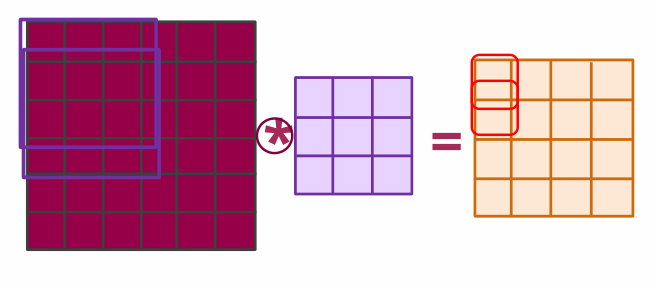
\includegraphics[width=\textwidth]{images/2dconvolutioneg1.png}
    \caption{Convolution Operation Denoted by \textbf{*}}
\end{figure}

\subsection{Image Filtering for Noise Reduction}
We typically use \textbf{smoothing} to remove \textit{high-frequency noise} without unduly damaging the larger \textit{low-frequency} objects of interest.
Commonly used smoothing filters include:
\begin{itemize}
    \item   \textbf{Blur:} averages a pixel and its neighbours.
    \item   \textbf{Median:} replaces a pixel with the median (rather than the mean) of the pixel and its neighbours.
    \item   \textbf{Gaussian:} a filter that produces a smooth response (unlike blur/``box'' \& median filtering) by weighting more towards the centre.
\end{itemize}

A typical ``classical'' (pre-deep learning) computer vision pipeline consists of the following steps:
\begin{enumerate}
    \item   Clean-up / Pre-processing:
            \begin{itemize}
                \item   Reduce noise (smoothing kernels).
                \item   Remove geometric/radiometric distortion.
                \item   Emphasise desired aspects of the image, e.g., edges, corners, blobs, etc. (differentiating kernels, feature detectors).
            \end{itemize}

    \item   Segmentation:
            \begin{itemize}
                \item   Identify / extract objects of interest.
                \item   Sometimes the entire image is of interest, so the task is to separate it into non-overlapping regions.
                \item   Most likely leverages domain-specific knowledge.
                \item   Not always needed in deep learning based approaches.
            \end{itemize}

    \item   Measurement:
            \begin{itemize}
                \item   Quantify appropriate measurements on segmented objects.
                \item   Might not be needed in deep learning based approaches.
            \end{itemize}

    \item   Classification:
            \begin{itemize}
                \item   Assign segmented objects to classes.
                \item   Make decision etc.
            \end{itemize}
\end{enumerate}

\subsection{Image Filtering for Edge Detection}
Consider a horizontal slice across the image: \textbf{edge detection} filters are essentially performing a differentiation of the grey level with respect to distance, i.e., ``how different is a pixel to its neighbours?''.
Some filters are akin to \textit{first derivatives} while others are more akin to \textit{second derivatives}.
\\\\
\textbf{Edge detection} is a common early step in image segmentation (often preceded by noise reduction).
Edge detection determines how different pixels are from their neighbours: abrupt changes in brightness are interpreted as the edges of objects.
Differentiating kernels can represent \textbf{first order} or \textbf{second order} derivatives.
Differentiating kernels for edge detection can also be classified as \textbf{gradient magnitude} or \textbf{gradient direction}.

\subsubsection{First Order Derivatives}
The general image processing pipeline is as follows:
\[
    \text{Smoothing (to reduce noise)} \rightarrow \text{Derivative (so that noise is not accentuated)}
\]

Most differentiating kernels are built by combining these two operations.
First order derivatives include:
\begin{itemize}
    \item   1D Gaussian derivative kernels.
    \item   2D Gaussian derivative kernels: image gradients
            \[
                \nabla f(x,y) = \left[ \frac{\partial f}{\partial x} \frac{\partial f}{\partial y} \right]^T
            \]
\end{itemize}

In image processing, an image can be represented as a 2D function $I(x,y)$ where $x$ \& $y$ are spatial co-ordinates and $I$ is the pixel intensity at those co-ordinates.
The first-order derivatives in the $x$- \& $y$-directions are defined as:
\[
    \frac{\partial I}{\partial x} \text{ and } \frac{\partial I}{\partial y}
\]
These derivatives measure the rate of change of intensity in the horizontal \& vertical directions respectively.
The concept is the same as differentiating a function, but applied to discrete pixel values, usually using finite differences or convolution with derivative filters.
\\\\
The \textbf{Prewitt operator} is the simplest 2D differentiating kernel.
It is obtained by convolving a 1D Gaussian derivative kernel with a 1D box filter in the orthogonal direction.
It is used to estimate the gradient of an image's intensity by highlighting regions with high spatial intensity variation, making it useful for detecting edges \& boundaries.
It uses two $3 \times 3$ convolution kernels to approximate the first-order derivatives of the image in the horizontal \& vertical directions.

\begin{align*}
    \text{Prewitt}_x =& \frac{1}{3} 
    \begin{bmatrix}
        1 \\
        1 \\
        1
    \end{bmatrix}
    \otimes
    \frac{1}{2}
    \begin{bmatrix}
        1 & 0 & -1
    \end{bmatrix}
    =
    \frac{1}{6}
    \begin{bmatrix}
        1 & 0 & -1 \\
        1 & 0 & -1 \\
        1 & 0 & -1
    \end{bmatrix} \\
    \text{Prewitt}_y =& \frac{1}{3} 
    \begin{bmatrix}
        1 & 1 & 1
    \end{bmatrix}
    \otimes
    \frac{1}{2}
    \begin{bmatrix}
        1 \\
        0 \\
        -1
    \end{bmatrix}
    =
    \frac{1}{6}
    \begin{bmatrix}
        1 & 0 & -1 \\
        1 & 0 & -1 \\
        1 & 0 & -1
    \end{bmatrix}
\end{align*}

The \textbf{Sobel operator} is more robust than the Prewitt operator as it uses the Gaussian $\sigma^2 = 0.5$ for the smoothing kernel:
\begin{align*}
    \text{Sobel}_x =& \text{gauss}_{0.5}(y) \otimes \text{gauss}_{0.5}(x)
    = \frac{1}{4}
    \begin{bmatrix}
        1 \\
        2 \\
        1
    \end{bmatrix}
    \otimes
    \frac{1}{2}
    \begin{bmatrix}
        1 & 0 & -1
    \end{bmatrix}
    = \frac{1}{8}
    \begin{bmatrix}
        1 & 0 & -1 \\
        2 & 0 & -2 \\
        1 & 0 & 1
    \end{bmatrix} \\
    \text{Sobel}_y =& \text{gauss}_{0.5}(x) \otimes \text{gauss}_{0.5}(y)
    = \frac{1}{4}
    \begin{bmatrix}
        1 & 2 & 1
    \end{bmatrix}
    \otimes
    \frac{1}{2}
    \begin{bmatrix}
        1 \\
        0 \\
        -1
    \end{bmatrix}
    = \frac{1}{8}
    \begin{bmatrix}
        1 & 2 & 1 \\
        0 & 0 & 0 \\
        -1 & -2 & -1
    \end{bmatrix}
\end{align*}

The \textbf{Scharr operator} is similar to the Sobel operator but with a smaller variance $\sigma^2 = 0.375$ in the smoothing kernel.

\begin{tcolorbox}[colback=gray!10, colframe=black, title=\textbf{Magnitude Images using First Order Derivatives}]
    Calculate ``magnitude images'' of the directional image gradients in the following image:
\begin{figure}[H]
    \centering
    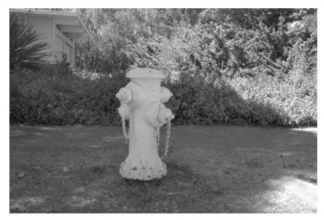
\includegraphics[width=0.4\textwidth]{images/magnitudeimagesone.png}
    \caption{Example Image}
\end{figure}

\begin{multicols}{2}

\begin{figure}[H]
    \centering
    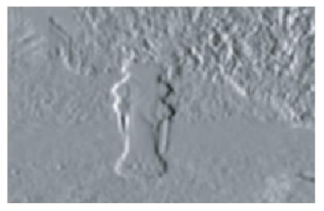
\includegraphics[width=0.4\textwidth]{images/magnitudeimagestwo.png}
    \caption{Partial Derivative in the $x$ Direction}
\end{figure}

\begin{figure}[H]
    \centering
    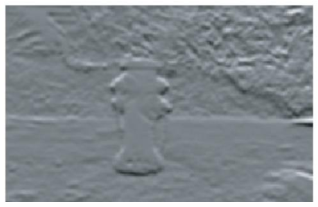
\includegraphics[width=0.4\textwidth]{images/magnitudeimagesthree.png}
    \caption{Partial Derivative in the $y$ Direction}
\end{figure}

\begin{figure}[H]
    \centering
    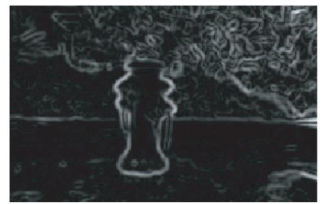
\includegraphics[width=0.4\textwidth]{images/magnitudeimagesfour.png}
    \caption{The Magnitude of the Gradient}
\end{figure}

\begin{figure}[H]
    \centering
    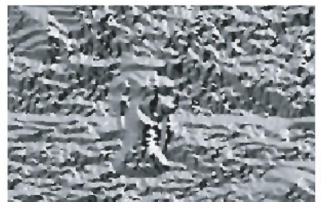
\includegraphics[width=0.4\textwidth]{images/magnitudeimagesfive.png}
    \caption{The Phase of the Gradient}
\end{figure}
\end{multicols}

The partial derivatives of the image in the $x$ \& $y$ directions together form the two components of the gradient of the image.
\end{tcolorbox}

\begin{tcolorbox}[colback=gray!10, colframe=black, title=\textbf{Edge Detection by Thresholding Magnitude Images}]
    Calculate edges by thresholding ``magnitude images'' of the directional image gradients.

\begin{figure}[H]
    \centering
    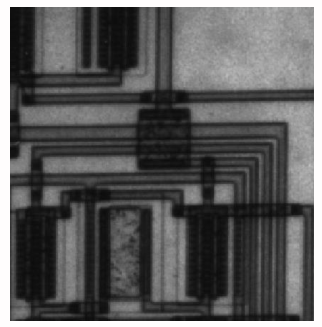
\includegraphics[width=0.3\textwidth]{images/thresholdingmagnitudeimages1.png}
    \caption{Input Greyscale Image}
\end{figure}

\begin{figure}[H]
    \centering
    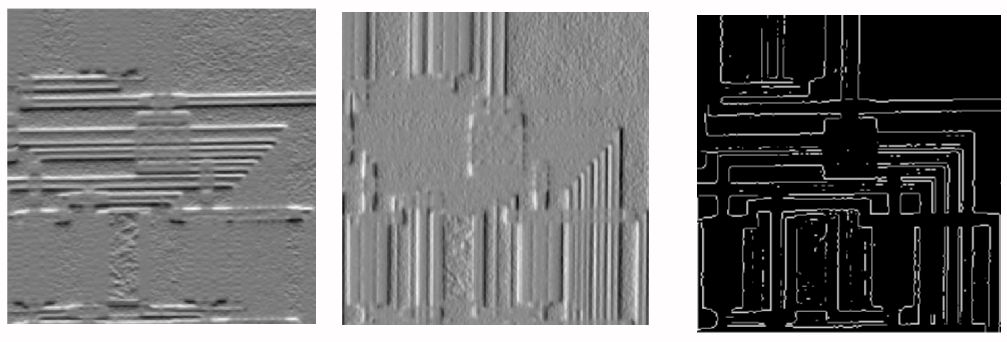
\includegraphics[width=\textwidth]{images/thresholdingmagnitudeimages2.png}
    \caption{Prewitt Operator (Vertical Gradient, Horizontal Gradient, Thresholding Gradient Magnitude)}
\end{figure}
\begin{figure}[H]
    \centering
    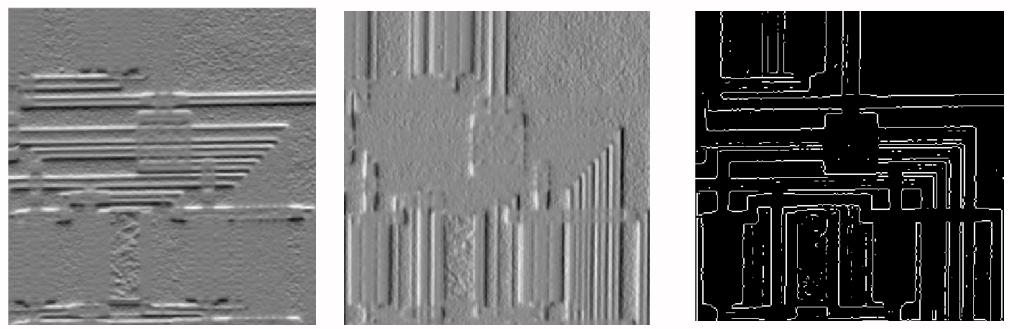
\includegraphics[width=\textwidth]{images/thresholdingmagnitudeimages3.png}
    \caption{Sobel Operator (Vertical Gradient, Horizontal Gradient, Thresholding Gradient Magnitude)}
\end{figure}
\end{tcolorbox}

\subsubsection{Second Order Derivatives}
For a function (or image) of two variables, the \textbf{second order derivative} in the $x$ \& $y$ directions can be obtained by convolving with the appropriately oriented \textbf{second-derivative kernel}.
For a function or image $I(x,y)$, the second-order derivatives measure how the rate of change of the function changes, represented by $\frac{\partial^2 I(x,y)}{\partial x^2}$ for the second derivative in the $x$-direction and $\frac{\partial^2 I(x,y)}{\partial y^2}$ for the second derivative in the $y$-direction.
\\\\
In image processing, second-order derivatives can be computed using specialised convolution kernels that act as second-derivative operators:
\begin{align*}
    \frac{\partial^2 I(x,y)}{\partial x^2} =& I(x,y) \otimes
    \begin{bmatrix}
        1 & -2 & 1
    \end{bmatrix}\\
    \frac{\partial^2 I(x,y)}{\partial y^2} =& I(x,y) \otimes
    \begin{bmatrix}
        1 \\
        -2 \\
        1
    \end{bmatrix}
\end{align*}

These kernels detect changes in intensity by convolving with the image.
When applied, they help identify where the intensity values change significantly, highlighting potential edges or other features.
\\\\
These kernels are second-order derivatives because they involve convolving the function with a differentiating kernel twice.
This can be seen in 1D by convolving the function with the non-centralised difference operator, then convolving the result again with the same operator:
\[
    (f(x) \otimes \begin{bmatrix}1 & -1\end{bmatrix} \otimes \begin{bmatrix} 1 & -1 \end{bmatrix}) = f(x) \otimes (\begin{bmatrix} 1 & -1 \end{bmatrix} \otimes \begin{bmatrix} 1 & 01 \end{bmatrix}) = f(x) \otimes \begin{bmatrix} 1 & -2 & 1 \end{bmatrix}
\]

Note that these 2D derivatives are not isotropic or symmetric.

COME BACK TO LAPLACIAN OPERATOR

\subsection{Image Filtering in the Frequency Domain}
Any signal, discrete or continuous, periodic or non-periodic, can be represented as a sum of sinusoidal waves of different frequencies and phases which constitute the frequency domain representation of that signal.

\section{Morphological Image Processing}
The term \textbf{morphology} refers to shape.
Morphological image processing assumes that an image consists of structures that can be handled by mathematical set theory.
It is normally applied to binary (black \& white) images, e.g. after applying thresholding.
A \textbf{set} is a group of pixels; different set operations can be performed on this set of pixels.
Applications for morphological image analysis generally involve image analysis at a very small scale (i.e., small regions of pixels) e.g., medical image processing, scientific image processing, industrial inspection, etc.

\begin{figure}[H]
    \centering
    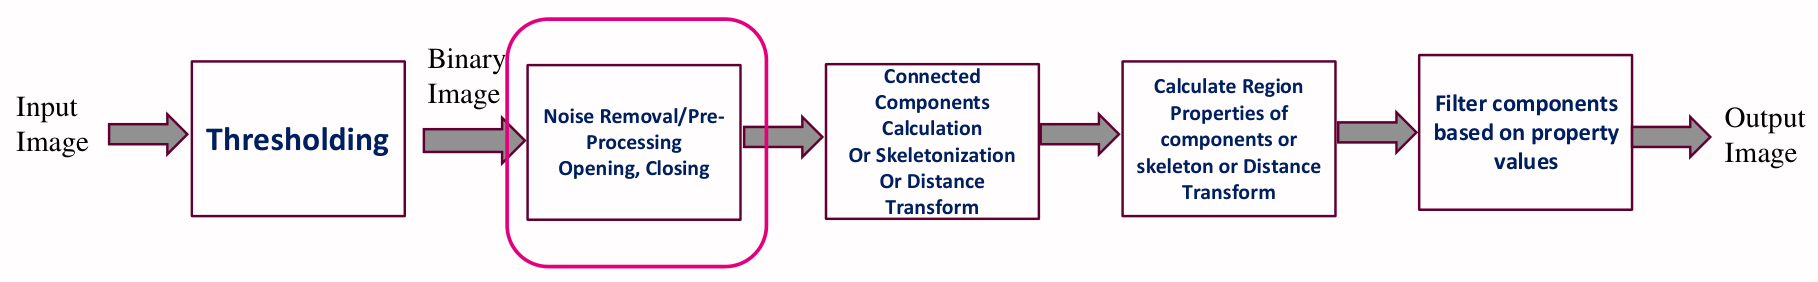
\includegraphics[width=\textwidth]{images/generalmorphologicalimageprocessingpipeline.png}
    \caption{A General Morphological Image Processing Pipeline}
\end{figure}

\begin{figure}[H]
    \centering
    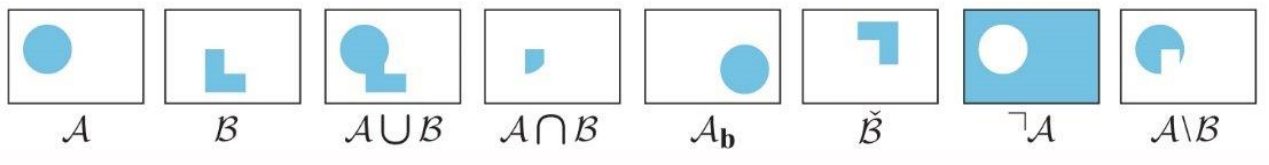
\includegraphics[width=\textwidth]{images/basicsetoperators.png}
    \caption{Basic Set Operators (From left to right: union, intersection, shift of $A$ by some amount $b$, reflection about the origin (assumed to be at the center), complement, \& set difference)}
\end{figure}

We can describe morphological differences in terms of intersections with test sets called \textbf{structuring elements (SEs)}.
SEs are of a much smaller size than the original image.
Morphological operations transform an image, i.e. changing a pixel from black to white (or vice-versa) if a defined structuring element ``fits'' at that point.
The shape + size of the structuring element directly affect the information about the image obtained by the operation.

\begin{tcolorbox}[colback=gray!10, colframe=black, title=\textbf{Structuring Elements Example}]
\begin{figure}[H]
    \centering
    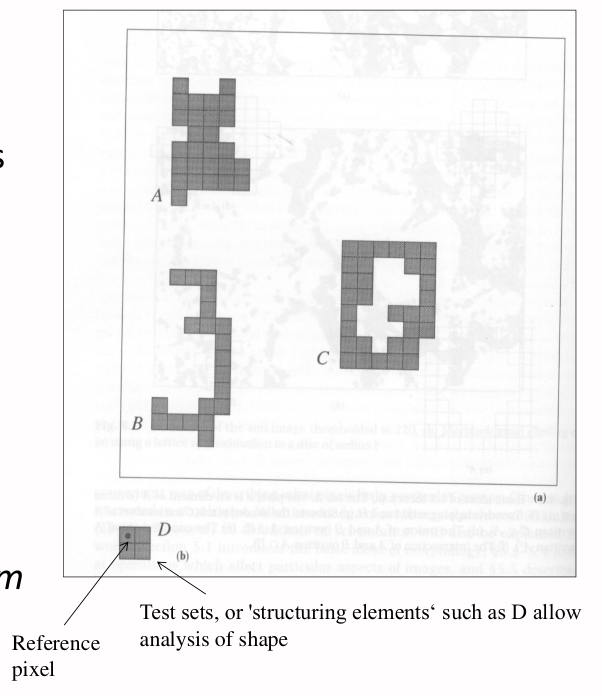
\includegraphics[width=0.5\textwidth]{images/seexample.png}
    \caption{Structuring Elements Example}
\end{figure}

The three black objects $A$, $B$, \& $C$ are very similar in size (i.e., number of pixels) but different in morphology/shape.
E.g., several possible translations of $D$ will fit into A, but none will fit into $B$.
\end{tcolorbox}

\subsection{Basic Morphological Operations}
Basic morphological operations are performed by set operations between a given image and a structuring element, e.g., erosion, dilation, opening, closing.

\begin{figure}[H]
    \centering
    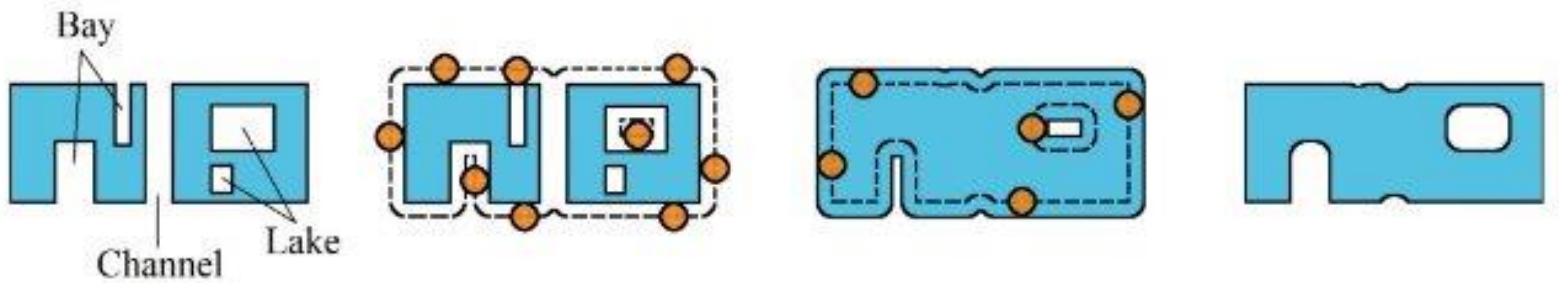
\includegraphics[width=\textwidth]{images/dilationofbinaryregion.png}
    \caption{
        Dilation of a binary region by a circular structuring element can be visualised as rolling the disk along the outside of the region; the result is enclosed by the path of the centre of the disk.
        The right column shows the result of \textit{closing} (dilation followed by erosion), which fills lakes, bays, \& channels.
    }
\end{figure}

\begin{figure}[H]
    \centering
    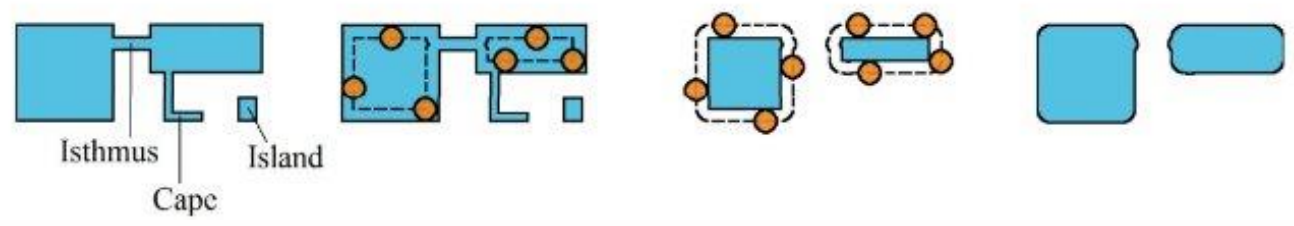
\includegraphics[width=\textwidth]{images/erosiionofbinaryregion.png}
    \caption{
        Erosion can be visualised as rolling the disk along the inside of the region; the result is again enclosed by the path of the centre of the disk.
        The right column shows the result of \textit{opening} (erosion followed by dilation), which removes capes, isthmuses, \& islands.
    }
\end{figure}

\begin{figure}[H]
    \centering
    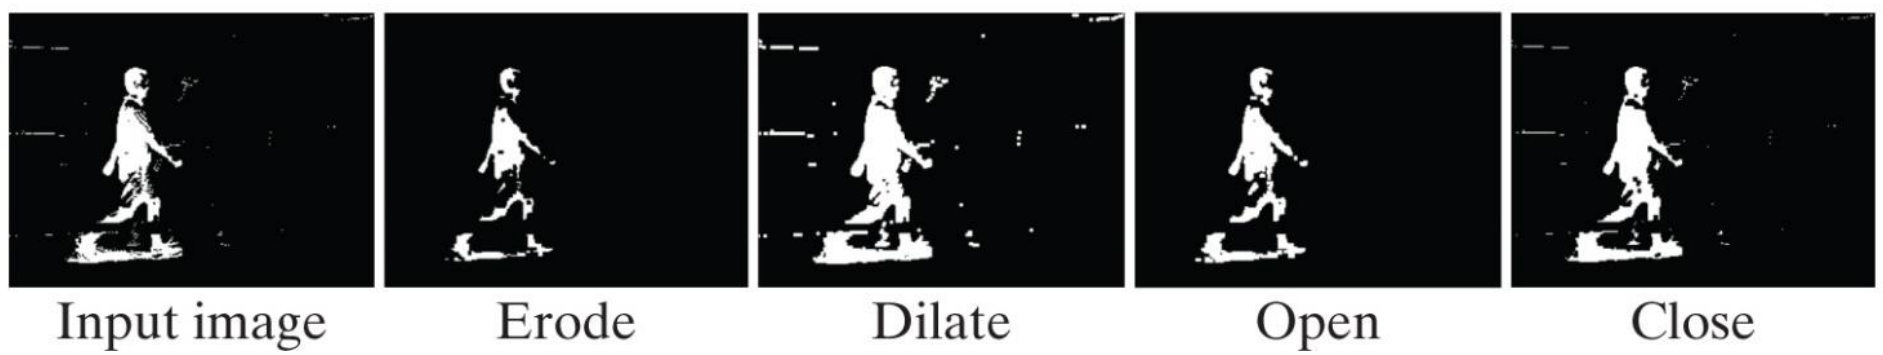
\includegraphics[width=\textwidth]{images/resultofmorphologicaloperations.png}
    \caption{
        A binary image and the result of morphological operations: erode, dilate, open, \& close.
        Erosion removes salt noise but shrinks the foreground.
        Dilate fills pepper noise but expands the foreground.
        Opening \& closing removes the respective types of noise while retaining the overall size of the foreground.
    }
\end{figure}

\textbf{Thinning} is an operation used to reduce objects in a binary image to their skeletons without breaking their connectivity.
It progressively removes pixels from the edges of objects while maintaining the general structure \& topology.
It can be thought of as ``clever erosion'' and is done by using crafter ternary structuring elements (on, off, don't care).

\begin{figure}[H]
    \centering
    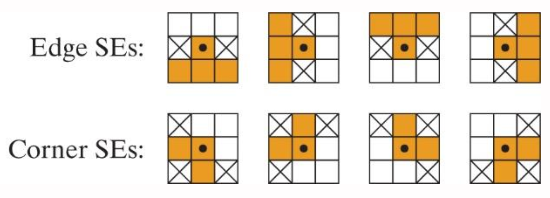
\includegraphics[width=0.8\textwidth]{images/thinningSEs.png}
    \caption{
        Structuring elements commonly used for morphological thinning.
        Coloured pixels are \textsc{on}, white pixels are \textsc{off}, and X indicates \textsc{don't-care}.
        The top row shows the four edge SEs, while the bottom row shows the four corner SEs.
    }
\end{figure}

\begin{figure}[H]
    \centering
    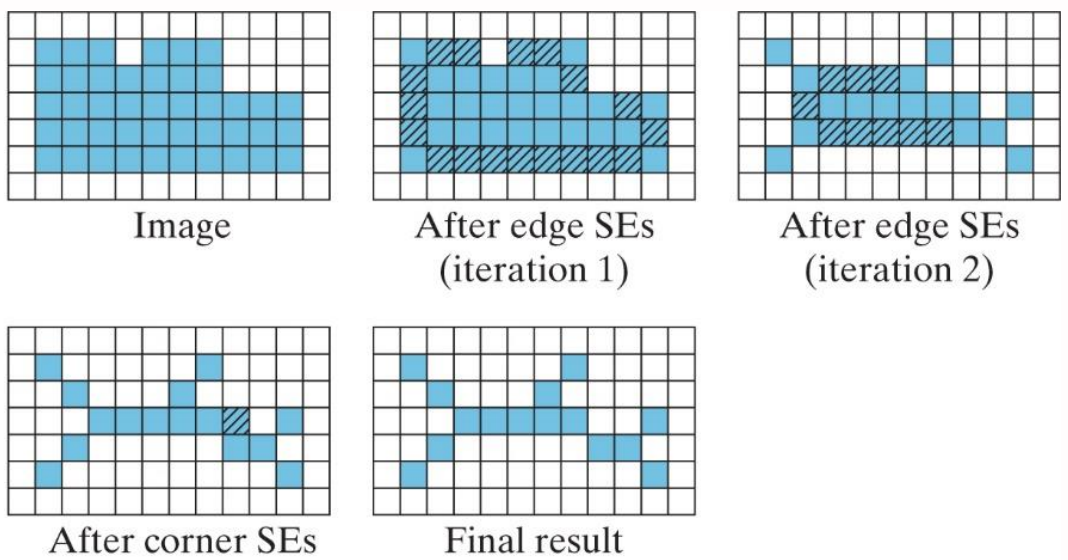
\includegraphics[width=0.8\textwidth]{images/thinningofsameimageusingSEs.png}
    \caption{
        Morphological thinning of the same binary image using the same SEs as the previous example.
        In this case, however, the edge SEs are applied repeatedly as a set until convergence, before applying the corner SEs repeatedly as a sequence.
        In the first iteration, pixels along the top, right, bottom, \& left of the region are removed by the edge SEs.
        In the second iteration, nine additional pixels are removed by the edge SEs.
        In the final iteration, a single pixel is removed by one of the corner SEs, thus producing a thinner skeleton than in the previous example.
    }
\end{figure}

\textbf{Thickening} is the opposite of thinning, i.e. adding pixels to the foreground.
\begin{figure}[H]
    \centering
    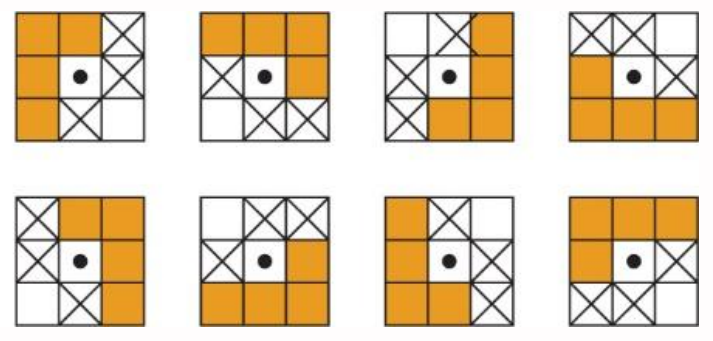
\includegraphics[width=0.8\textwidth]{images/thickeningSEs.png}
    \caption{
        Structuring elements commonly used for morphological thickening.
    }
\end{figure}

\begin{figure}[H]
    \centering
    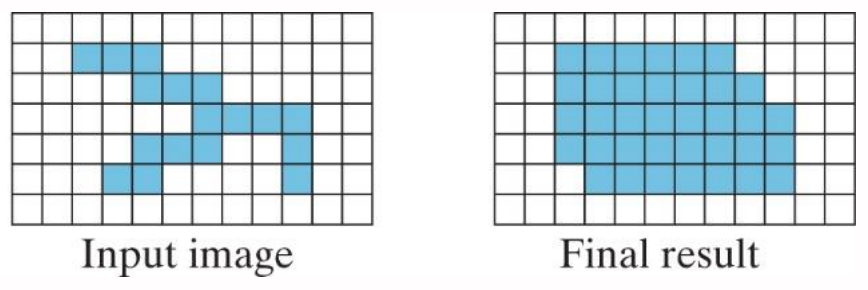
\includegraphics[width=0.8\textwidth]{images/thickeningSEsbinaryexample.png}
    \caption{
        Morphological thickening of a binary image using the SEs above.
        Shown are the original image (left) and the final result after convergence (right).
        The thickened result is an approximation to the convex hull.
    }
\end{figure}

\begin{figure}[H]
    \centering
    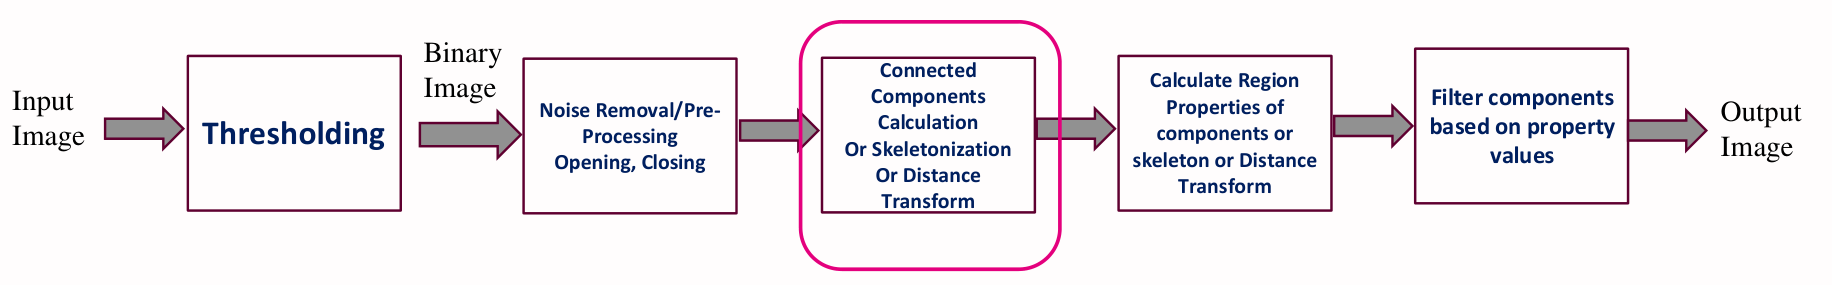
\includegraphics[width=\textwidth]{images/morphimagepipeline.png}
    \caption{ A general morphological image processing pipeline. }
\end{figure}

\subsection{Connected Components}
A pixel $q = (q_x, q_y)$ is a neighbour of pixel $p = (p_x, p_y)$ if $q$ is in the \textbf{neighbourhood} of $p$, denoted $q \in N(p)$ where $N$ is the neighbourhood function.
Two pixels are said to be \textbf{adjacent} if they have the same value and if they are neighbours of each other.
Pixels are said to be \textbf{connected} or \textbf{contiguous} if there exists a path between them

\begin{figure}[H]
    \centering
    \includegraphics[width=0.6\textwidth]{images/commonneighbourhoods.png}
    \caption{Commonly used neighbourhoods. From left to right: $N_4$, $N_8$, \& $N_D$.}
\end{figure}

\begin{figure}[H]
    \centering
    \includegraphics[width=0.6\textwidth]{images/binaryregioncommonneighbourhoods.png}
    \caption{A binary region and the 4-, 8-, \& $m$-adjacency of its pixels. Note that $m$-adjacency removes the loops that sometimes occur with 8-adjacency.}
\end{figure}

A \textbf{connected component} is defined as a maximal set of pixels that are all connected with one another.
\textbf{Connected component labelling} is the process of assigning a unique identifier to every pixel in the image indicating the connected component to which it belongs.

\subsection{Distance Transform}
A \textbf{distance transform} replaces pixels of one value (black or white) in a binary image with their distance to the nearest pixel of opposite value (white or black).
This is useful for template matching \& granulometry (studying the size distribution/properties of objects).
The assumption is that a local maximum is the centre of a distinct object: use a ``non-maximal suppressin'' to remove all other pixels.

\begin{figure}[H]
    \centering
    \includegraphics[width=0.4\textwidth]{images/distancetransform.png}
    \caption{Distance Transform Example}
\end{figure}

\subsection{Skeletonisation}
A common approach to \textbf{skeletonisation} is to repeatedly thin the image until the result converges.
\begin{figure}[H]
    \centering
    \includegraphics[width=0.6\textwidth]{images/skeletonisation.png}
    \caption{The skeleton of a binary region is defined as the locus of points where the wave fronts of fires set to the boundary meet, or equivalently as the locus of the centres of the maximal balls.}
\end{figure}

\begin{figure}[H]
    \centering
    \includegraphics[width=0.8\textwidth]{images/skeletonisationexamples.png}
    \caption{Six different continuous shapes (blue) and their skeletons (red).}
\end{figure}

\begin{figure}[H]
    \centering
    \includegraphics[width=0.8\textwidth]{images/skeletonisationalgorithms.png}
    \caption{Comparison of the various skeletonisation algorithms on two different binary images.}
\end{figure}

\subsection{Region Properties}
\textbf{Regular moments} are statistical measures calculated from the pixel intensity values of an image that help in understanding the distribution of pixel values and can be used for shape analysis.
The $p^\text{th}$ moment is defined as:
\[
    m_{pq} = \sum_x \sum_y x^p y^q I(x,y)
\]
where $I(x,y)$ is the pixel intensity at co-ordinates $(x,y)$.
\\\\
\textbf{Central moments} are similar to regular moments but are computed with respect to the mean of the pixel distribution.
They provide a measure of the shape's properties such as its variance.
The $p^\text{th}$ central moment is defined as:
\[
    \mu_{pq} = \sum_x \sum_y (x - \overline{x})^p (y - \overline{y})^q I(x,y)
\]
where $\overline{x}$ \& $\overline{y}$ are the mean co-ordinates.
\\\\
The \textbf{covariance matrix} is used to describe the distribution of points in a shape.
It captures the relationship between the dimensions of the shape and is crucial for understanding the orientation \& spread of the shape in the feature space.
\[
    C =
    \begin{bmatrix}
        \mu_{20} & \mu_{11} \\
        \mu_{11} & \mu_{02}
    \end{bmatrix}
\]

\textbf{Compactness} is defined as:
\[
    \text{compactness} = \frac{4\pi (\text{area})}{(\text{perimeter})^2}
\]

\begin{figure}[H]
    \centering
    \includegraphics[width=0.8\textwidth]{images/compactness.png}
    \caption{
        Left: a circle is the most compact shape, with a compactness of 1.
        Middle: a shape whose compactness is less than 1.
        Right: the eccentricity of the shape is computed as the eccentricity of the best-fitting ellipse.
    }
\end{figure}

The \textbf{convex hull} of a region is the shape that results from enveloping the region with a rubber band, which removes all concavities.

\begin{figure}[H]
    \centering
    \includegraphics[width=0.6\textwidth]{images/convexhull.png}
    \caption{
        Left: An arbitrarily shaped region in the plane.
        Right: The convex hull of the region.
        All vertices in both regions are locally convex except for $p_2$.
    }
\end{figure}

\textbf{Eccentricity} measures the elongatedness of a binary region, i.e., how far it is from being rotationally symmetric around its centroid.
To calculate it the eccentricity of a binary region:
\begin{enumerate}
    \item   Find the best/tightest fitting ellipse around the region.
    \item   Then align this ellipse with the axes.
    \item   Find the Covariance Matrix of this ellipse:
            \[
                C = P
                \begin{bmatrix}
                    \lambda_1 & 0 \\
                    0 & \lambda_2
                \end{bmatrix}
                P^T
            \]
            This covariance matrix is obtained by using the moments of the binary region encapsulated by the ellipse:
            \[
                C = \frac{1}{\mu_{00}}
                \begin{bmatrix}
                    \mu_{20} & \mu_{11} \\
                    \mu{11} & \mu_{02}
                \end{bmatrix}
                =
                \eta
                \begin{bmatrix}
                    c & - \frac{b}{2} \\
                    -\frac{b}{2} & a
                \end{bmatrix}
            \]

    \item   The eccentricity will be a ratio of the eigenvalues of this matrix:
            \[
                \text{eccentricity} = \sqrt{\frac{\lambda_1 - \lambda_2}{\lambda_1}}
            \]
\end{enumerate}

\textbf{Topology} is the study of objects that are preserved under continuous deformations of the objects, e.g., bending, stretching, \& compressing but not tearing or sewing.
\textbf{Homotopy} or rubber sheet deformations is defined to be a deformation which does not change the topology of the object.

\begin{figure}[H]
    \centering
    \includegraphics[width=0.6\textwidth]{images/homotopy.png}
    \caption{
        Top: the letters ``A'' \& ``P'' are related by a homotopy because there is a continuous deformation that relates the two shapes.
        Bottom: the letters ``A'' \& ``B'' are not related by a homotopy because there is not a continuous deformation that relates the two shapes.
        Rather, tearing the region to produce the extra hole is necessary (or sewing the hole in the case of the reverse transformation).
    }
\end{figure}

The \textbf{Euler number} is a topological invariant characteristic defined by:
\begin{align*}
    \text{Euler number} =& \text{number of regions} - \text{number of holes} \\
                        =& \text{number of vertices} - \text{number of edges} + \text{number of faces}
\end{align*}

\begin{figure}[H]
    \centering
    \includegraphics[width=0.6\textwidth]{images/eulertesselations.png}
    \caption{
        Various tessellations of a region whose Euler number is 1 (left) and 0 (right), showing that the Euler number is not dependent upon the particular tessellation chosen.
        Under each figure is the number of vertices minus edges plus faces according to the formula for the Euler number.
        Note that there is implicitly at least one vertex, edges intersect at vertices, \& external vertices or edges are not counted.
    }
\end{figure}

\textbf{Region boundary representations} are classically used in ``shape'' analysis or recognition.
For distinguishing the shape of the boundary, generally we want to transform the sequence into a representation that is invariant to translation, rotation, and/or scale changes, as well as to the starting pixel.
The most basic type of \textbf{signature} s known as the \textbf{centroidal profile} or \textbf{$r$-$\theta$ curve}.
This approach captures the distance $r$ from the centre of the region as a function of the angle $\theta$.

\begin{figure}[H]
    \centering
    \includegraphics[width=0.6\textwidth]{images/centroidalprofile.png}
    \caption{The centroidal profile ($r$-$\theta$ plot) of several shapes}
\end{figure}

\section{Edge \& Feature Detection}
\subsection{Multiresolution Processing}
\textbf{Multiresolution} refers to analysing the image at mutliple resolutions (scales).
A $40 \times 40$ region in the original image will occupy only a $20 \times 20$ region in the downsampled image, a $10\times10$ region in the twice downsampled image, and so forth.
Because each successive image is smaller than its predecessor, stacking the images on top of one another yields the shape of a pyramid called an \textbf{image pyramid}.
Image pyramids are created by smoothing $\rightarrow$ downsampling $\rightarrow$ smoothing $\rightarrow$ downsampling.
\\\\
A \textbf{Gaussian pyramid} is when the image is smoothed by convolving with a Gaussian kernel.
\begin{align*}
    I^{(0)} (x,y)  =& I(x,y) \\
    I^{(i+1)}(x,y) =& \left( I^{(i)} (x,y) \circledast \text{Gauss}_{\sigma^2} (x,y) \right) \downarrow 2
\end{align*}

\begin{figure}[H]
    \centering
    \includegraphics[width=0.6\textwidth]{images/gaussianpyramids.png}
    \caption{
        Twelve levels of a Gaussian pyramid, obtained with $\sigma^2 = \frac{1}{4}(0.5) = 0.125$ and a downsampling factor of $\sqrt[4]{2}$.
        Note that $I^{(4)}$ is half as large as $I^{(0)}$ in each direction, and that $I^{(8)}$ is half as large as $I^{(4)}$.
    }
\end{figure}

A \textbf{Laplacian pyramid} is when the image is smoothed by convolving with several Gaussian kernels of varying variance, then taking their Difference of Gaussian (DoG) to approximate Lapalacian of Gaussian (LoG).
\[
    L^{(i+1)} (x,y) = \left( I^{(0)} (x,y) \circledast \text{LoG}_{(i+1)\sigma^2} (x,y) \right) \downarrow (i + 1) d
\]

\begin{figure}[H]
    \centering
    \includegraphics[width=0.6\textwidth]{images/laplacianpyramids.png}
    \caption{
        Laplacian pyramid with $n = 2$ images per octave.
        THe images are successively convolved with a Gaussian, then downsampled at the end of each octave to produce something that closely resembles a Gaussian pyramid.
        Differences between successive Gaussian-smoothed images yield DoGs, which approximate LoGs.
        The initial variance is $\frac{1}{2} (0.5) = 0.25$ and the ratio between successive standard deviations is $\rho = \sqrt{2}$.
    }
\end{figure}

To construct a series of images at different \textbf{scale-spaces}, an image is convolved with varying kernel sizes of Gaussian smooting kernels of varying size \& variance (``scale'').
It can be seen as an embedding of the original image into a one-parameter family of Gaussian kernels of increasing variance -- being the \textbf{continuous parameter}.
The image size remains the same and is not down-sampled.
It is used in further image analysis techniques such as SIFT Features.

\begin{figure}[H]
    \centering
    \includegraphics[width=0.6\textwidth]{images/gaussianscalespace.png}
    \caption{
        The Gaussian scale space of an image consists of a continuous 3D volume in which each slice is an increasingly blurred version of the original image.
        Shown here are ten sample images from the scale space.
    }
\end{figure}

\subsection{Edge Detection}
\textbf{Intensity edges} are pixels in the image where the intensity (or grey level) function changes rapidly.
A \textbf{step edge} occurs when a light region is adjacent to  dark region.
A \textbf{line edge} occurs when a thing light (or dark) object, such as a wire, is in front of a dark (or light) background.
A \textbf{roof edge} occurs when the change is not in the lightness itself but rather in the derivative of the lightness.
A \textbf{rampe edge} occurs when the lightness changes slowly across a region.

\begin{figure}[H]
    \centering
    \includegraphics[width=0.6\textwidth]{images/intesnityedges.png}
    \caption{Four types of intensity edges}
\end{figure}

The \textbf{Canny edge detector} is a classic algorithm for detecting intensity edges in a greyscale image that relies on the gradient magnitude.
The algorithm involves three steps:
\begin{enumerate}
    \item   First, the gradient of the image is computed, including the magnitude \& phase.
    \item   Second, in \textbf{non-maximum suppression}, any pixel is set to zero whose gradient magnitude is not a local maximum in the direction of the gradient.
    \item   Finally, \textbf{edge linking} is performed to discard pixels without much support.
\end{enumerate}

The Canny edge detector is highly regarded for a number of reasons:
\begin{itemize}
    \item   It has a good ability to locate as many edges as possible.
    \item   It is relatively insensitive to noise.
    \item   There will be a minimal distance between its detected edges and the real edges, which is important when you want to measure or classify extracted objects.
    \item   It only gives one response to each edge.
\end{itemize}

\begin{figure}[H]
    \centering
    \includegraphics[width=0.6\textwidth]{images/cannyedgedetails.png}
    \caption{
        Top: an image and its partial derivatives in the $x$ \& $y$ directions.
        Bottom: the gradient magnitude \& phase of the image, along with the thresholded gradient magnitude.
    }
\end{figure}


\begin{figure}[H]
    \centering
    \includegraphics[width=0.6\textwidth]{images/cannynonmaxsuppression.png}
    \caption{
        Non-maximum suppression.
        The gradient direction (or phase) $\theta$ is quantised into one of four values, shown by the coloured wedges of the circle.
        The quantised phase governs which of the two neighbours to compare with the pixel.
        If the gradient magnitude of the pixel is not at least as great as both neighbours, then it is set to zero.
        This has the effect of thinning the edges, as shown in the inset.
    }
\end{figure}

\begin{figure}[H]
    \centering
    \includegraphics[width=0.6\textwidth]{images/cannyedgelinking.png}
    \caption{
        Edge linking with hysteresis, also known as double thresholding or hysteresis thresholding.
        Thresholding the gradient magnitude with the low threshold produces too many edge pixels (left), while thresholding the high threshold produces too few edge pixels (middle).
        Edge linking with hysteresis combines the benefits of both (right) to produce the final Canny edge detector output.
    }
\end{figure}

\subsection{Feature Detection}
An edge detector finds pixels with large gradient magnitude, whereas a \textbf{feature detector} finds pixels where the greyscale values \textit{vary locally in more than one direction}.
One of the common places for feature points is at corners.
Feature detection is frequently used in motion detection, object tracking, image registration, image stitchin, 3D modelling, optical flow, \& visual odometry/SLAM (robotics).

\begin{figure}[H]
    \centering
    \includegraphics[width=0.6\textwidth]{images/panaroma.png}
    \caption{Applications for feature detection include image registration, mosaics, stitching, \& panorama generation.}
\end{figure}

These features are typically hand-crafted as opposed to being discovered by deep learning pipelines.
Good features are scale-invariant \& rotation invariant.
\\\\
Recall the \textbf{covariance matrix} built from central moments whose eigenvalues were used to find orientation \& eccentricity of a binary region.
\begin{align*}
    C_{(2 \times 2)}    =& E\left[ (x - \overline{x})(x - \overline{x})^T \rho(x) \right]\\
    =& \frac{1}{\mu_{00}}
    \begin{bmatrix}
        \mu_{20} & \mu_{11} \\
        \mu_{11} & \mu_{02} 
    \end{bmatrix}
\end{align*}

We can then build a \textbf{gradient covariance matrix} or \textbf{autocorrelation matrix} from image gradients:
\begin{align*}
    Z = \sum_{x \in R} w(x)
    \begin{bmatrix}
        I^2_x(x) & I_x(x)I_y(x) \\
        I_x(x)I_y(x) & I^2_y(x)
    \end{bmatrix}
    =
    \begin{bmatrix}
        z_x & z_{xy} \\
        z_{xy} & z_y
    \end{bmatrix}
\end{align*}

Eigenvalues of the gradient covariance matrix indicate how the pixel values are varying in different directions.
Eigenvalues are inherently rotationally invariant.
If both eigenvalues are large, then the pixel values are varying in different directions.
If one eigenvalue is large, it indicates an edge with pixel values that are varying in one direction only.
\\\\
The \textbf{Harris corner detector} finds pixel values with large ``cornerness'' defines as:
\begin{align*}
    \text{cornerness} =& \text{det}(Z) - k (\text{trace}(Z))^2 \\
    =& z_x z_y - z_{xy}^2 - k (z_x + z_y)^2 \\
    =& \lambda_1 \lambda_2 - k(\lamda_1 + \lambda_2)^2
\end{align*}

The \textbf{Tomasi-Kanade/Shi-Tomasi detector} finds pixel values with large ``cornerness'' defined as:
\begin{align*}
    \text{cornerness} = \text{min}( \{ \lambda_1, \lambda_2 \}) = \lambda_2
\end{align*}

\subsection{Feature Descriptors}
A \textbf{feature descriptor} characterises detected features in a way that can be used for comparison across images.
These include: SIFT features, GLOH (Gradient Location \& Histogram), HOG (Histogram of Gradients), etc.


\end{document}
